\documentclass[10pt]{beamer}
\usepackage[english]{babel}
\usepackage[utf8]{inputenc}
\usepackage[T1]{fontenc}
\usepackage{helvet}
\usepackage{lipsum}  
\usepackage{graphicx,subfigure}
%-------------------------------------------------------
% INFORMATION IN THE TITLE PAGE
%-------------------------------------------------------

\newcommand{\cstitle}{\textbf{Detección \textit{in Silico} de Neoantígenos Utilizando Transformers y Transfer Learning en el Marco de Desarrollo de Vacunas Personalizadas para Tratar el Cáncer}
\subtitle[]{Tésis de doctorado}}
\newcommand{\cscourseCode}{Detección de Neoantígenos}
\newcommand{\csauthor}{MSc. Vicente Machaca Arceda}
\institute[UNSA]{Universidad Nacional de San Agustín}
\newcommand{\csemail}{vmachaca@utec.edu.pe}
\newcommand{\instituteabr}{UTEC}
\newcommand{\nameUp}{}
\date{2023}
\title[\cscourseCode]{\cstitle}
\author{\csauthor}
%%%%%%%%%%%%%%%%%

%-------------------------------------------------------
% CHOOSE THE THEME
%-------------------------------------------------------
\def\mycmd{0} % UNSA
\def\mycmd{1} % SALLE
%\def\mycmd{2} % UTEC
%-------------------------------------------------------

\if\mycmd0
\usepackage{csformat}
\newcommand{\chref}[3][blue]{\href{#2}{\color{#1}{#3}}}%

\fi

\if\mycmd1
\usetheme[]{Feather}
\newcommand{\chref}[2]{	\href{#1}{{\usebeamercolor[bg]{Feather}#2}} }
\fi

\if\mycmd2
\usetheme{UTEC2020}	
\newcommand{\chref}[3][blue]{\href{#2}{\color{#1}{#3}}}%
\fi

\newcommand{\1}{
	\setbeamertemplate{background}{
		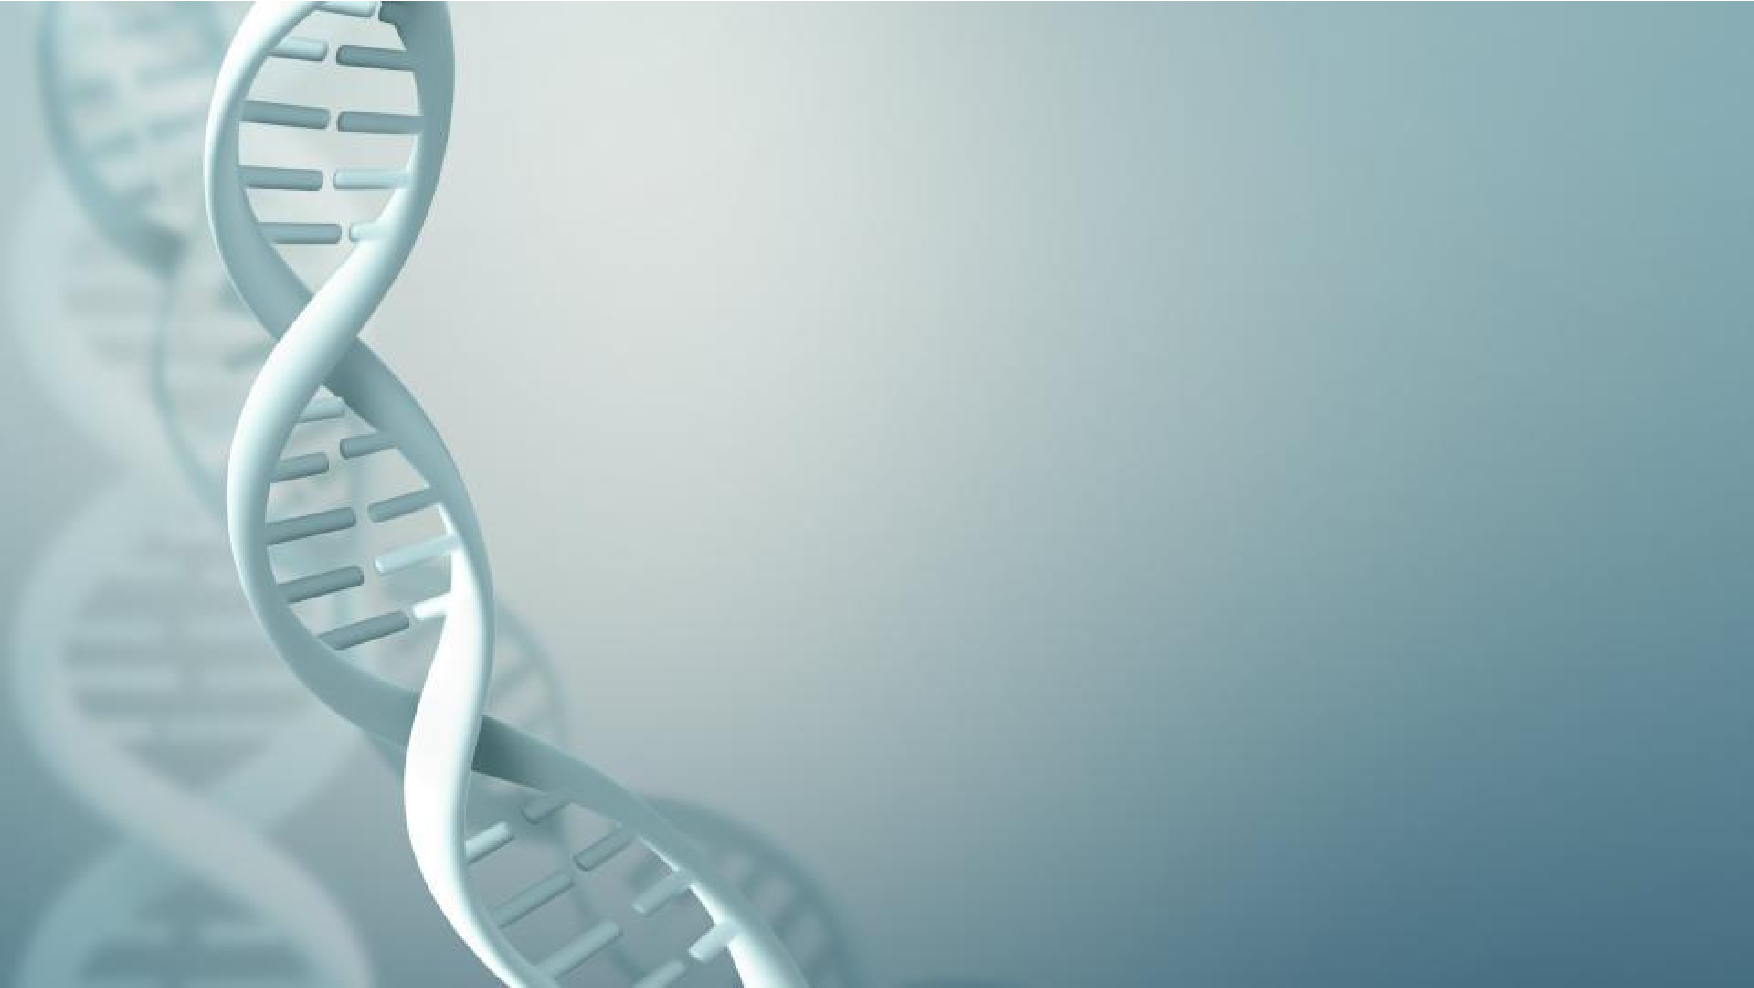
\includegraphics[width=\paperwidth,height=\paperheight]{img/1}
		\tikz[overlay] \fill[fill opacity=0.75,fill=white] (0,0) rectangle (-\paperwidth,\paperheight);
	}
}



%-------------------------------------------------------
% THE BODY OF THE PRESENTATION
%-------------------------------------------------------

\begin{document}
	
	
	\AtBeginSubsection[]
	{
		\begin{frame}
			\frametitle{Contenido}
			\tableofcontents[currentsubsection]
		\end{frame}
	}
	
	
	%-------------------------------------------------------
	% THE TITLEPAGE
	%-------------------------------------------------------
	
	\if\mycmd0
	\maketitle
	\fi
	
	\if\mycmd1 % MY THEME
	\1{
		\begin{frame}[plain,noframenumbering] 
			\titlepage 
	\end{frame}}
	\fi
	
	\if\mycmd2
	\begin{frame}
		\titlepage
	\end{frame}
	\fi
	%-------------------------------------------------------
	%-------------------------------------------------------


%-------------------------------------------------------
%-------------------------------------------------------
\begin{frame}{Contenido}
	\tableofcontents
\end{frame}
%-------------------------------------------------------
%-------------------------------------------------------


%%%%%%%%%%%%%%%%%%%%%%%%%%%%%%%%%%%%%%%%%%%%%%%%%%%%%%%%%%%%%%%%%%%%%%%%%%%%%%%%%%%%%%%%%%%%%%%%%%%%%%%%%%%%%%%%
%%%%%%%%%%%%%%%%%%%%%%%%%%%%%%%%%%%%%%%%%%%%%%%%%%%%%%%%%%%%%%%%%%%%%%%%%%%%%%%%%%%%%%%%%%%%%%%%%%%%%%%%%%%%%%%%
%%%%%%%%%%%%%%%%%%%%%%%%%%%%%%%%%%%%%%%%%%%%%%%%%%%%%%%%%%%%%%%%%%%%%%%%%%%%%%%%%%%%%%%%%%%%%%%%%%%%%%%%%%%%%%%%
\section{Contexto y Motivación}
%%%%%%%%%%%%%%%%%%%%%%%%%%%%%%%%%%%%%%%%%%%%%%%%%%%%%%%%%%%%%%%%%%%%%%%%%%%%%%%%%%%%%%%%%%%%%%%%%%%%%%%%%%%%%%%%
%%%%%%%%%%%%%%%%%%%%%%%%%%%%%%%%%%%%%%%%%%%%%%%%%%%%%%%%%%%%%%%%%%%%%%%%%%%%%%%%%%%%%%%%%%%%%%%%%%%%%%%%%%%%%%%%
%%%%%%%%%%%%%%%%%%%%%%%%%%%%%%%%%%%%%%%%%%%%%%%%%%%%%%%%%%%%%%%%%%%%%%%%%%%%%%%%%%%%%%%%%%%%%%%%%%%%%%%%%%%%%%%%

%%%%%%%%%%%%%%%%%%%%%%%%%%%%%%%%%%%%%%%%%%%%%%%%%%%%%%%%%%%%%%%%%%%%%%%%%%%%%%%%%%%%%%%%%%%%%%%%%%%%%%%%%%%%%%%%
\subsection{Estadísticas en Cáncer}
%%%%%%%%%%%%%%%%%%%%%%%%%%%%%%%%%%%%%%%%%%%%%%%%%%%%%%%%%%%%%%%%%%%%%%%%%%%%%%%%%%%%%%%%%%%%%%%%%%%%%%%%%%%%%%%%


%-------------------------------------------------------
%-------------------------------------------------------
\begin{frame}{Contexto y Motivación}{}
	\begin{block}{}
		An la actualidad, el cáncer representa el mayor problema de salud mundial \cite{siegel2023cancer}.
	\end{block}

	\begin{figure}[]
		\centering
		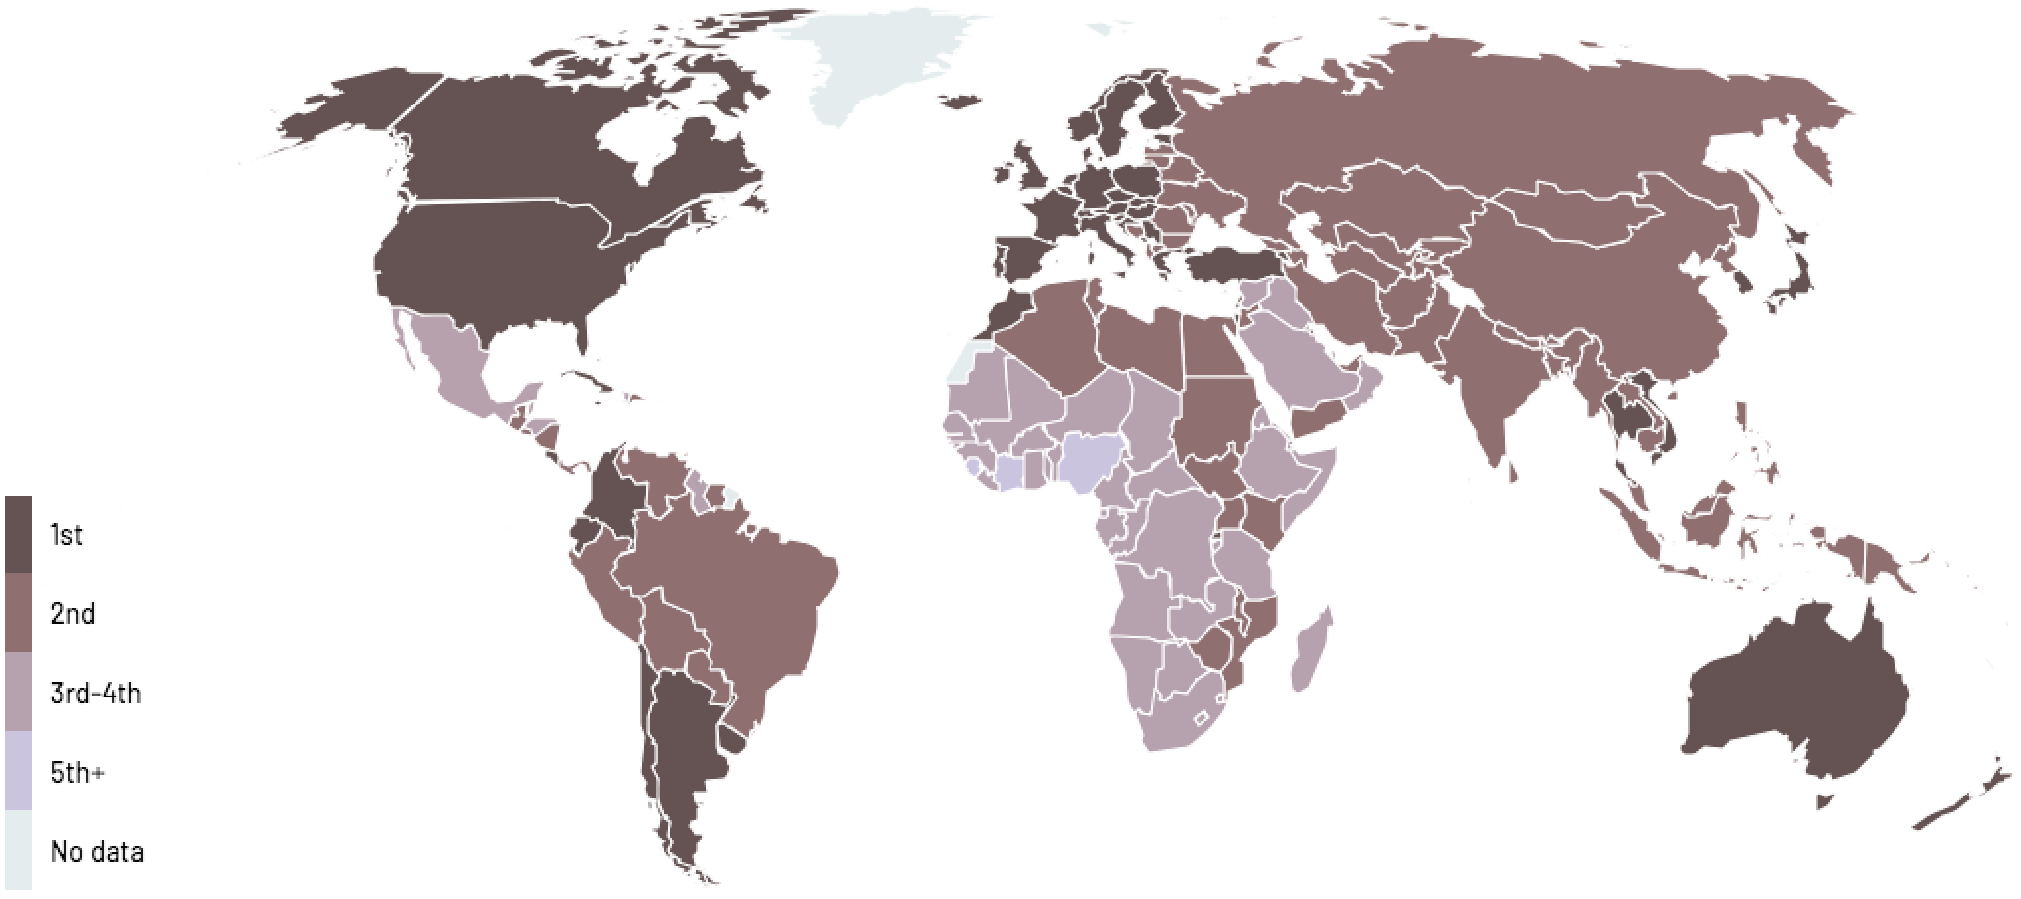
\includegraphics[width=\textwidth]{../img/introduction/cancer_deaths}
		\caption{Ranking de las muertes por cáncer entre 30 y 69 años. \textbf{Fuente}: The Atlas Cancer \cite{canceratlas2023}.}
	\end{figure}
\end{frame}
%-------------------------------------------------------
%-------------------------------------------------------

%-------------------------------------------------------
%-------------------------------------------------------
\begin{frame}{Contexto y Motivación}{Muertes por tipos de cáncer}
	\begin{figure}[]
		\centering
		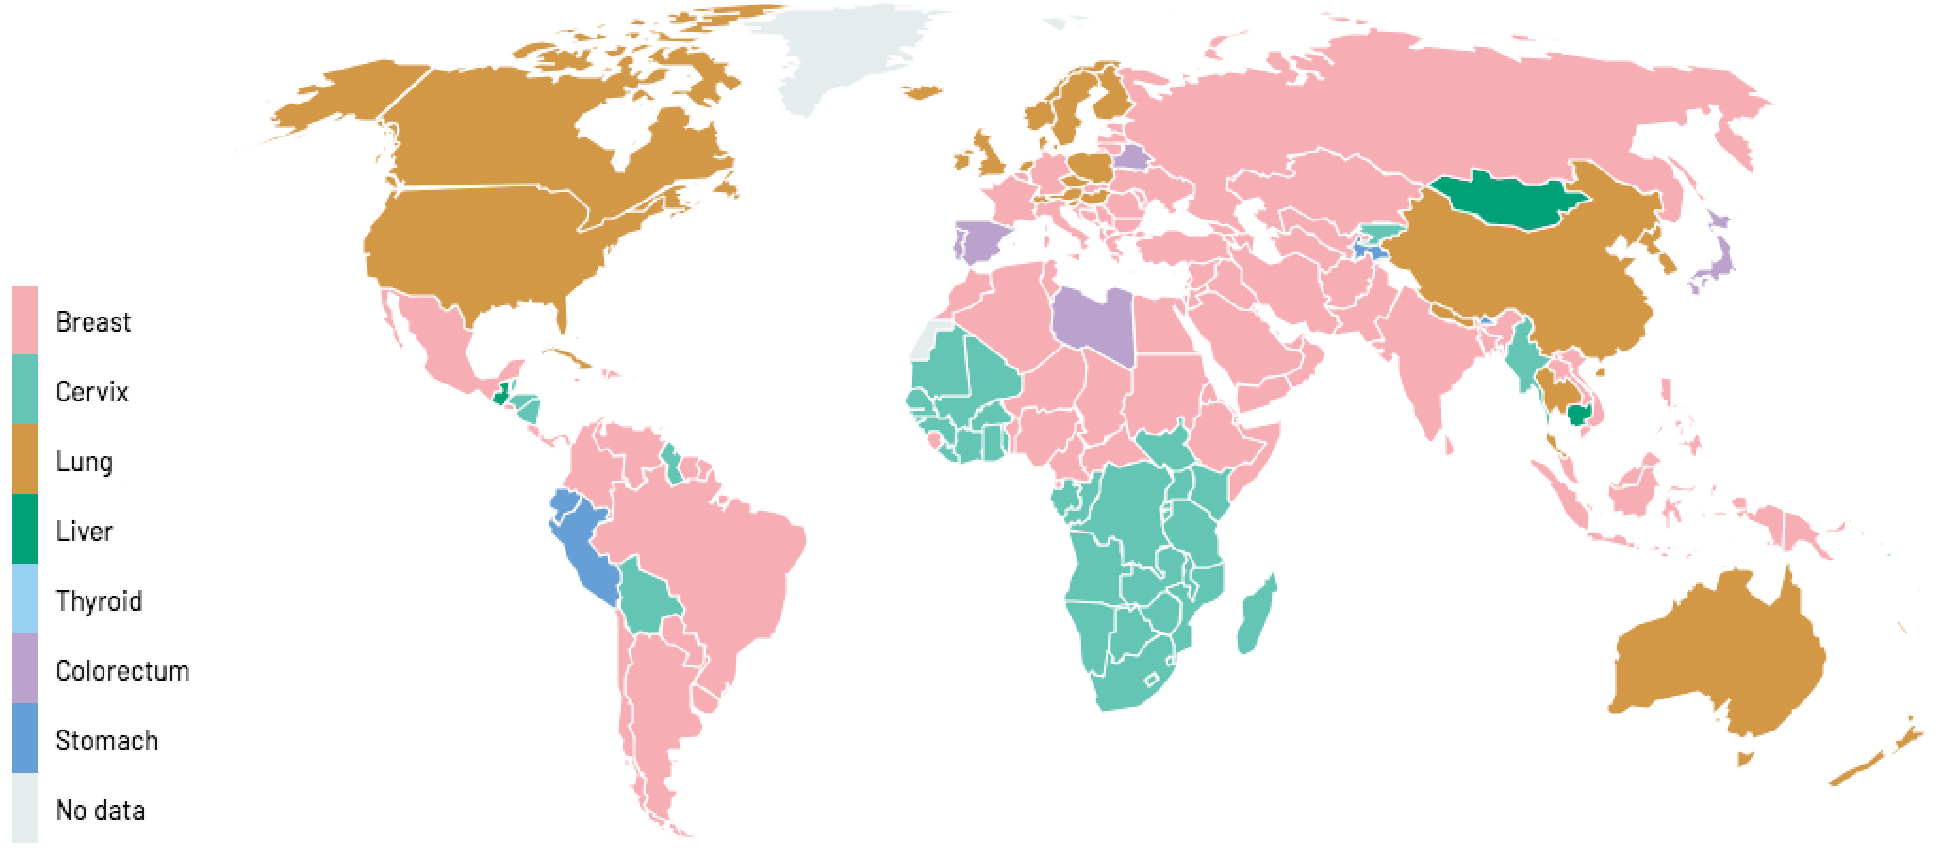
\includegraphics[width=\textwidth]{../img/introduction/cancer_deaths_woman}
		\caption{Ranking de las muertes por tipo de cáncer en mujeres. \textbf{Fuente}: The Atlas Cancer \cite{canceratlas2023}.}
	\end{figure}
\end{frame}
%-------------------------------------------------------
%-------------------------------------------------------


%-------------------------------------------------------
%-------------------------------------------------------
\begin{frame}{Contexto y Motivación}{Muertes por tipos de cáncer}
	\begin{figure}[]
		\centering
		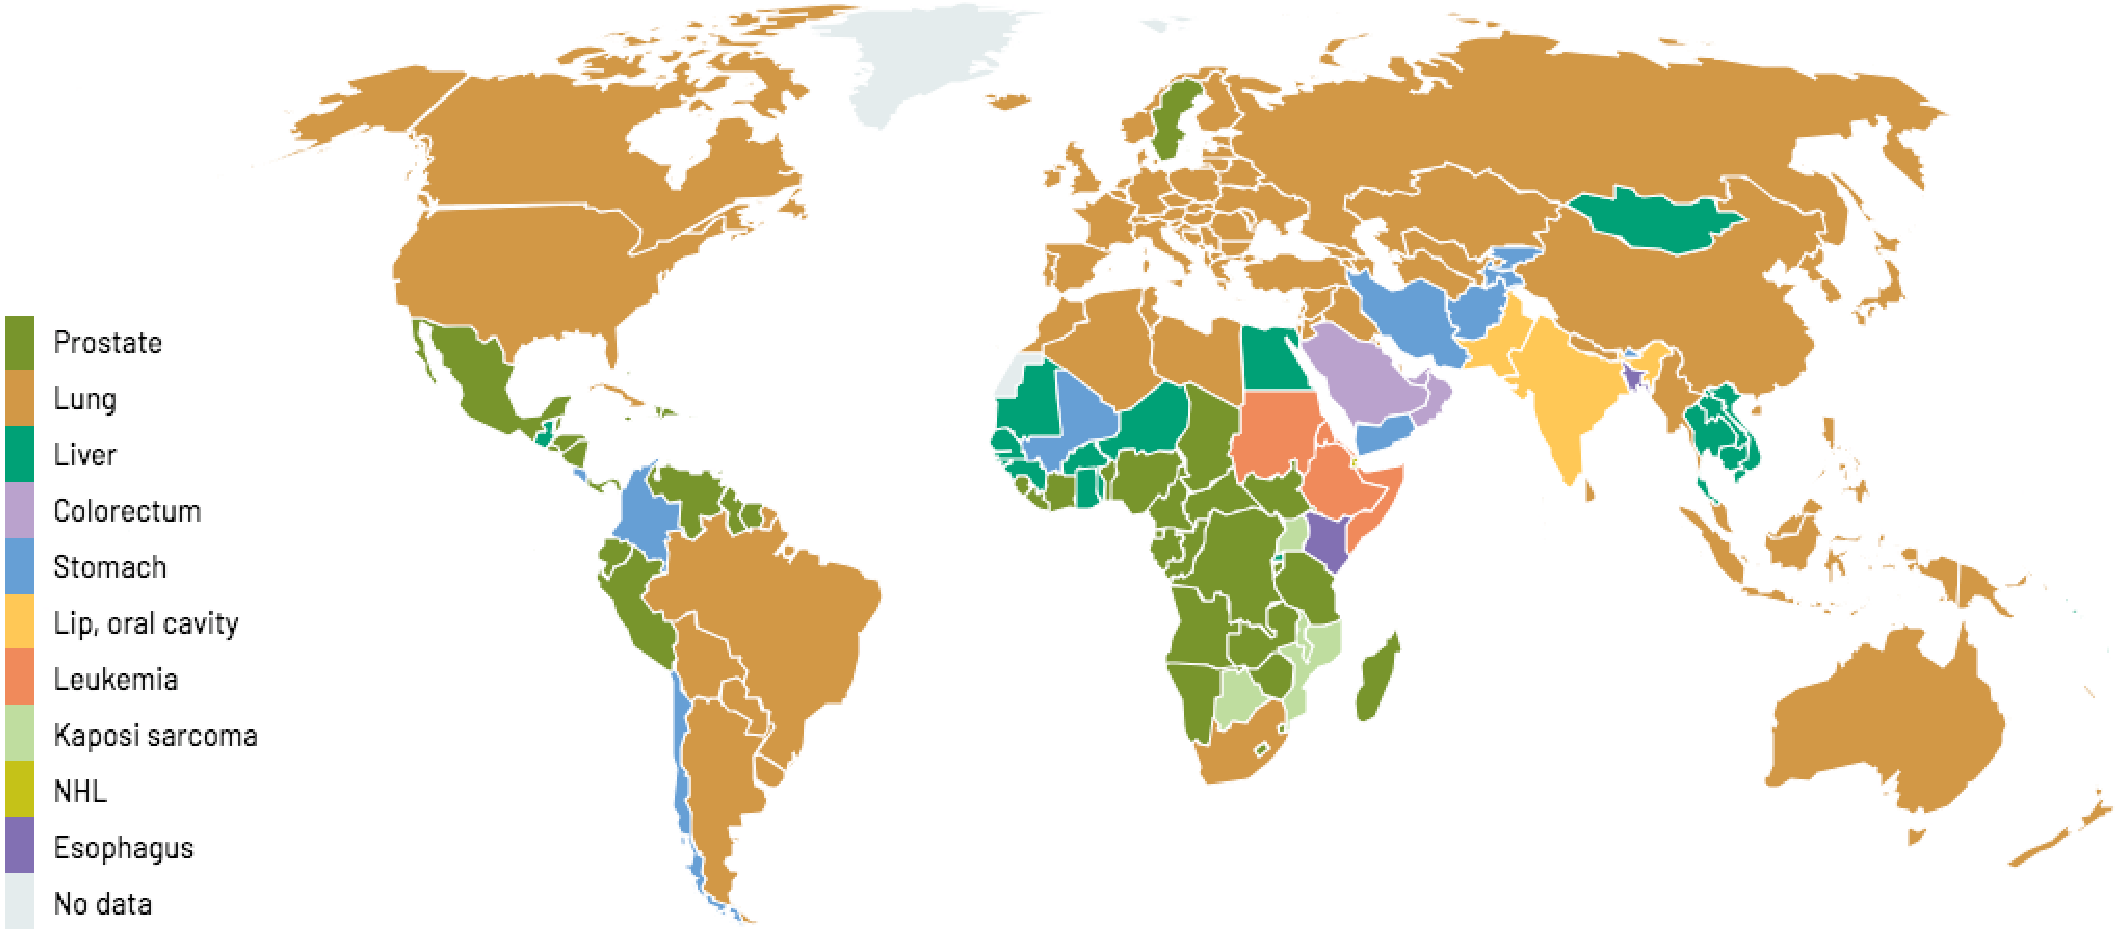
\includegraphics[width=\textwidth]{../img/introduction/cancer_deaths_man}
		\caption{Ranking de las muertes por tipo de cáncer en hombres. \textbf{Fuente}: The Atlas Cancer \cite{canceratlas2023}.}
	\end{figure}
\end{frame}
%-------------------------------------------------------
%-------------------------------------------------------


%-------------------------------------------------------
%-------------------------------------------------------
\begin{frame}{Contexto y Motivación}{Porcentaje de casos y muertes}
	\begin{figure}[]
		\centering
		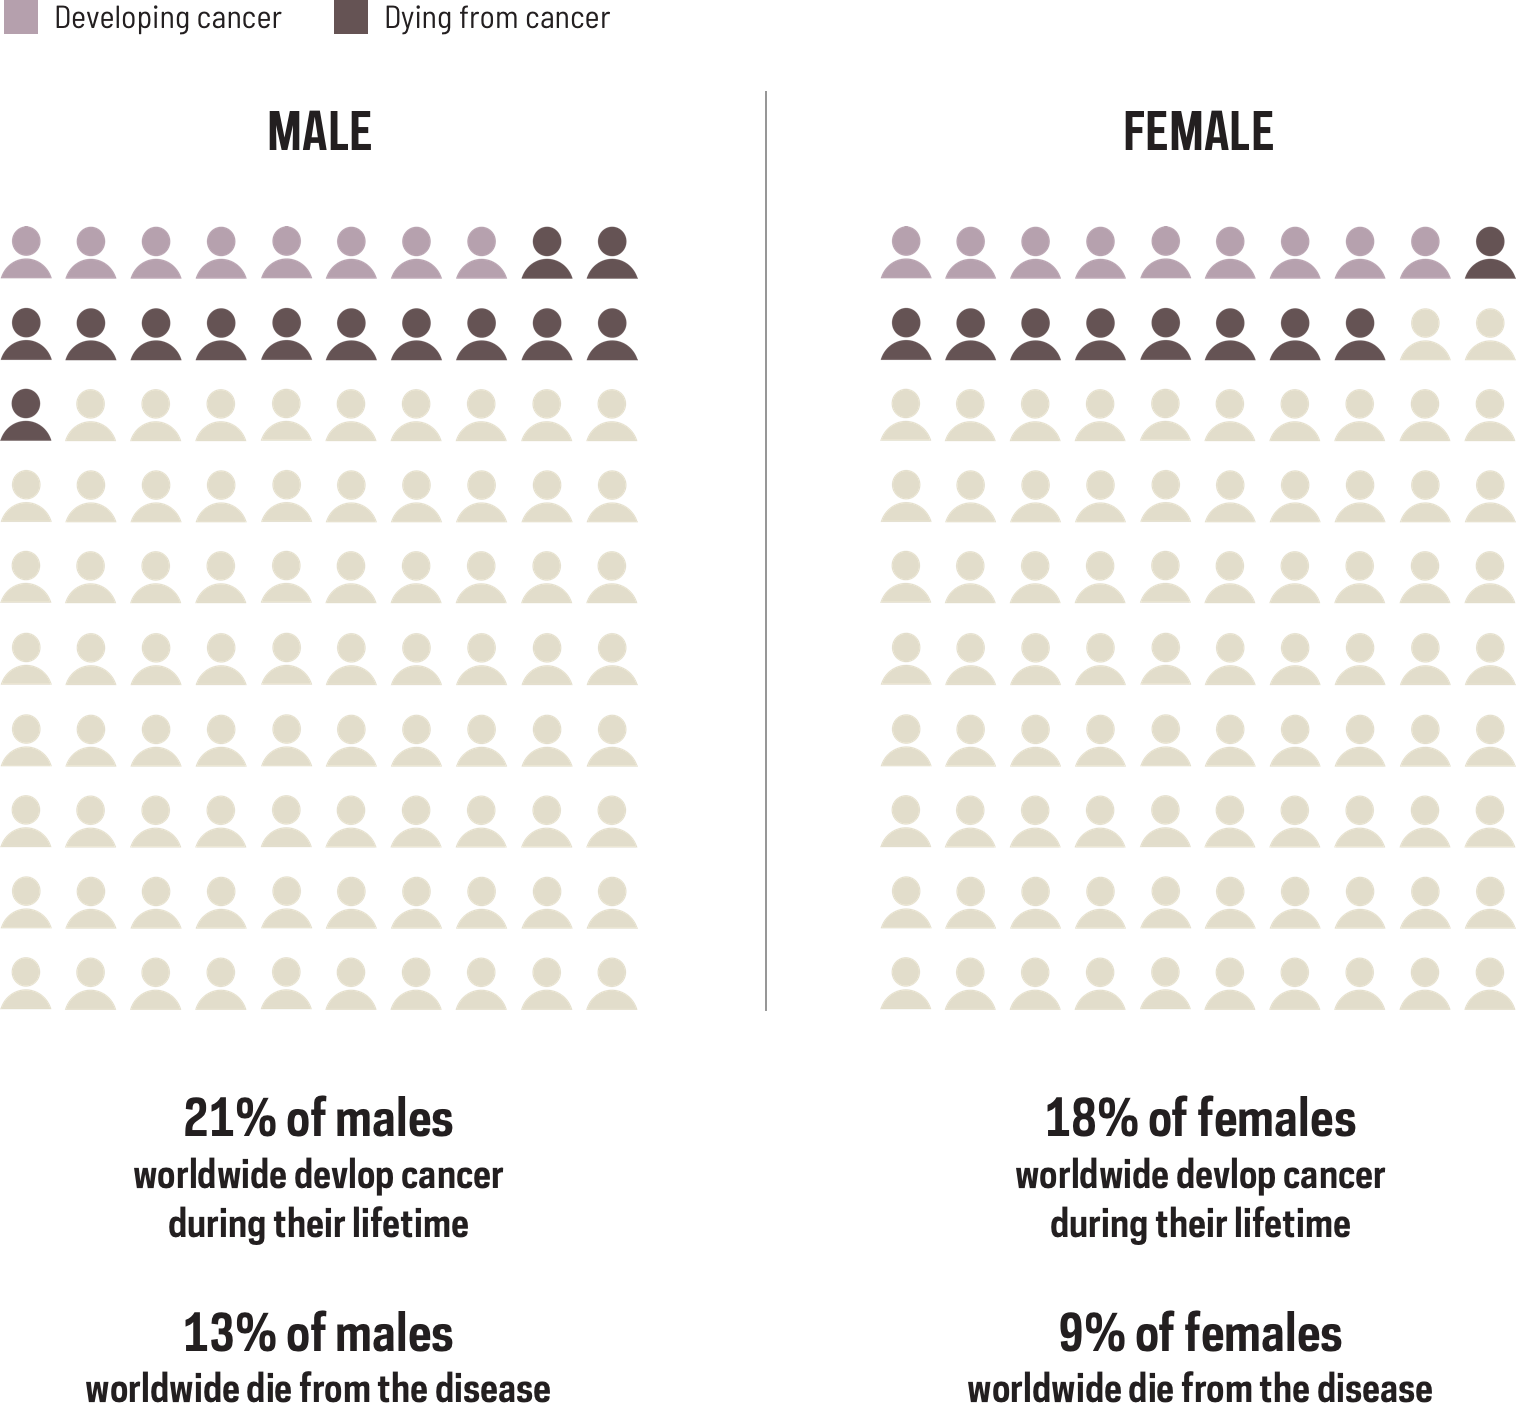
\includegraphics[width=0.6\textwidth]{../img/introduction/cancer_men_women}
		\caption{Porcentaje de casos y muertes por sexo. \textbf{Fuente} The Atlas Cancer \cite{canceratlas2023}.}
	\end{figure}
\end{frame}
%-------------------------------------------------------
%-------------------------------------------------------

%-------------------------------------------------------
%-------------------------------------------------------
\begin{frame}{Contexto y Motivación}{Predicción de nuevos casos}
	\begin{figure}[]
		\centering
		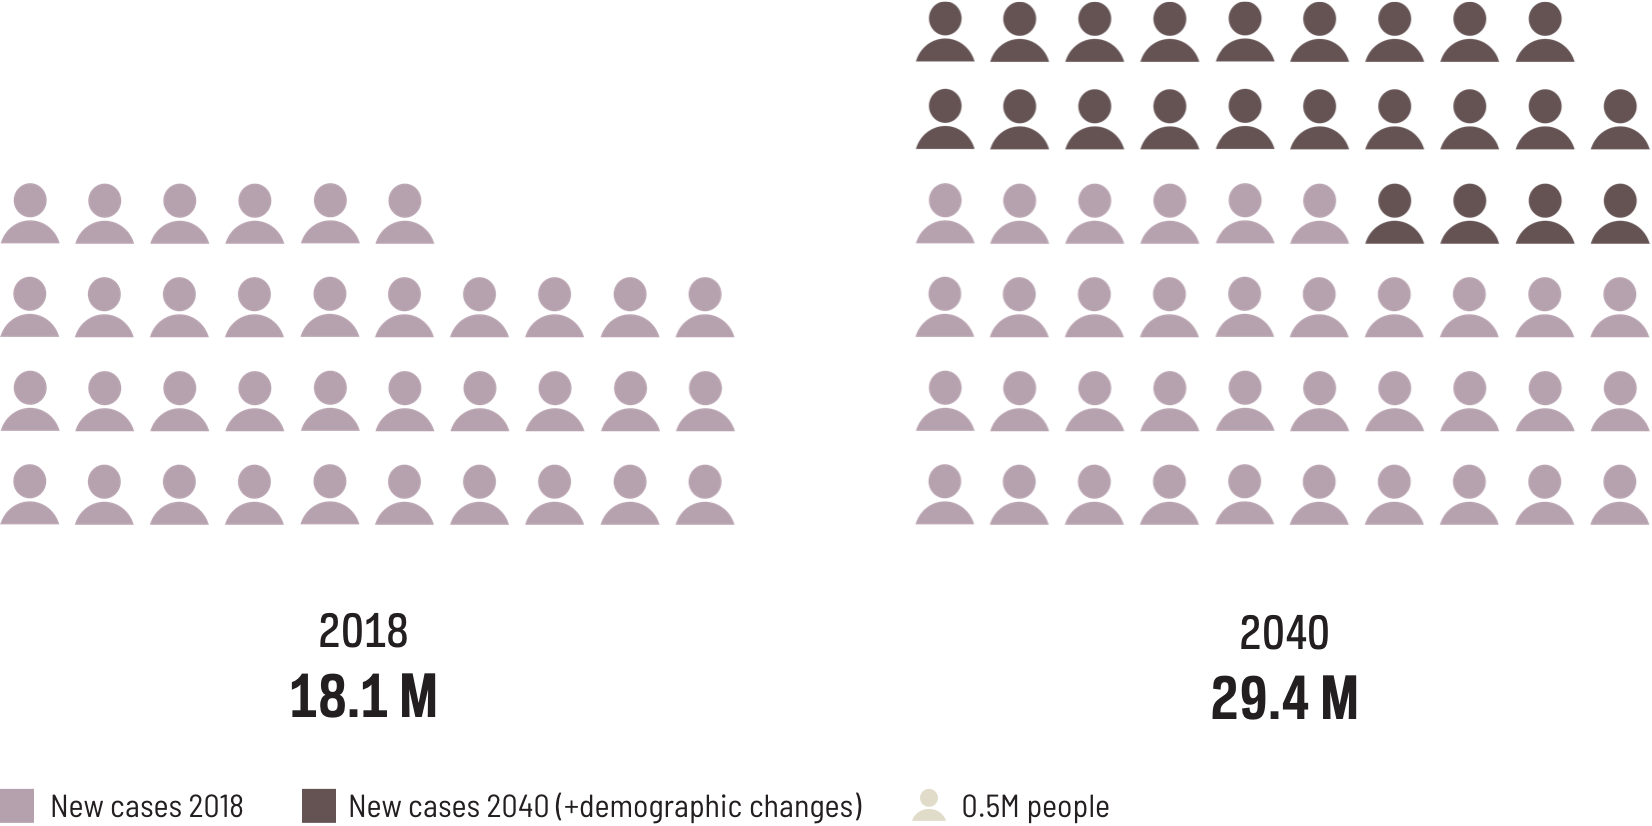
\includegraphics[width=\textwidth]{../img/introduction/cancer_new_cases}
		\caption{Predicción de nuevos casos para el 2040. \textbf{Fuente} The Atlas Cancer \cite{canceratlas2023}.}
	\end{figure}
\end{frame}
%-------------------------------------------------------
%-------------------------------------------------------

%%%%%%%%%%%%%%%%%%%%%%%%%%%%%%%%%%%%%%%%%%%%%%%%%%%%%%%%%%%%%%%%%%%%%%%%%%%%%%%%%%%%%%%%%%%%%%%%%%%%%%%%%%%%%%%%
\subsection{Inmunoterapia del Cáncer}
%%%%%%%%%%%%%%%%%%%%%%%%%%%%%%%%%%%%%%%%%%%%%%%%%%%%%%%%%%%%%%%%%%%%%%%%%%%%%%%%%%%%%%%%%%%%%%%%%%%%%%%%%%%%%%%%



%-------------------------------------------------------
%-------------------------------------------------------
\begin{frame}{Contexto y Motivación}{Reacciones distintas para cada paciente}
	%\begin{block}{}
	%	Pacientes con el mismo tipo de cáncer pueden reaccionar de forma disitinta a los mismos tratamientos.
	%\end{block}

	\begin{figure}[]
		\centering
		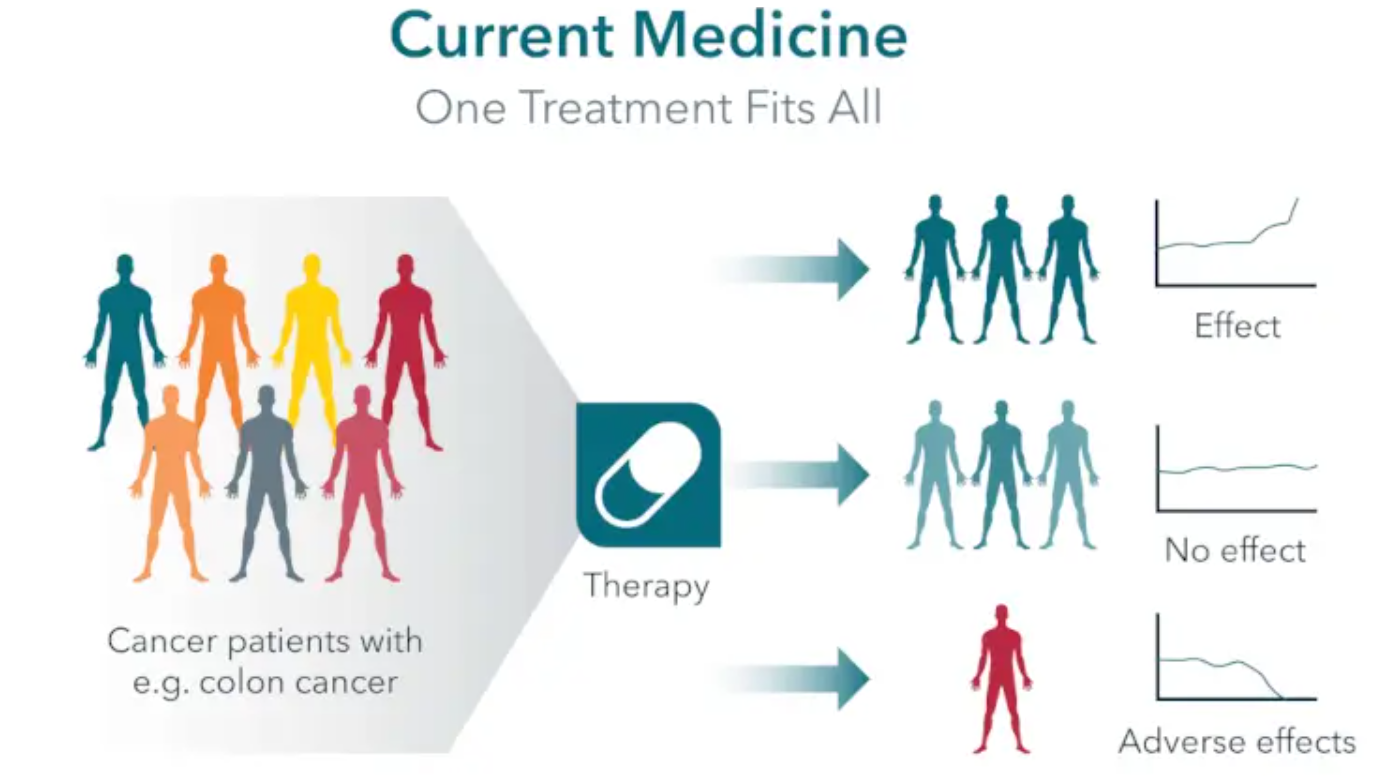
\includegraphics[width=\textwidth]{../img/introduction/medecine_current}
			\caption{Pacientes con el mismo tipo de cáncer pueden reaccionar de forma disitinta a los mismos tratamientos. \textbf{Fuente} The Atlas Cancer \cite{pdx2023}.}
	\end{figure}
\end{frame}
%-------------------------------------------------------
%-------------------------------------------------------

%-------------------------------------------------------
%-------------------------------------------------------
\begin{frame}{Contexto y Motivación}{Reacciones distintas para cada paciente}

	
	\begin{figure}[]
		\centering
		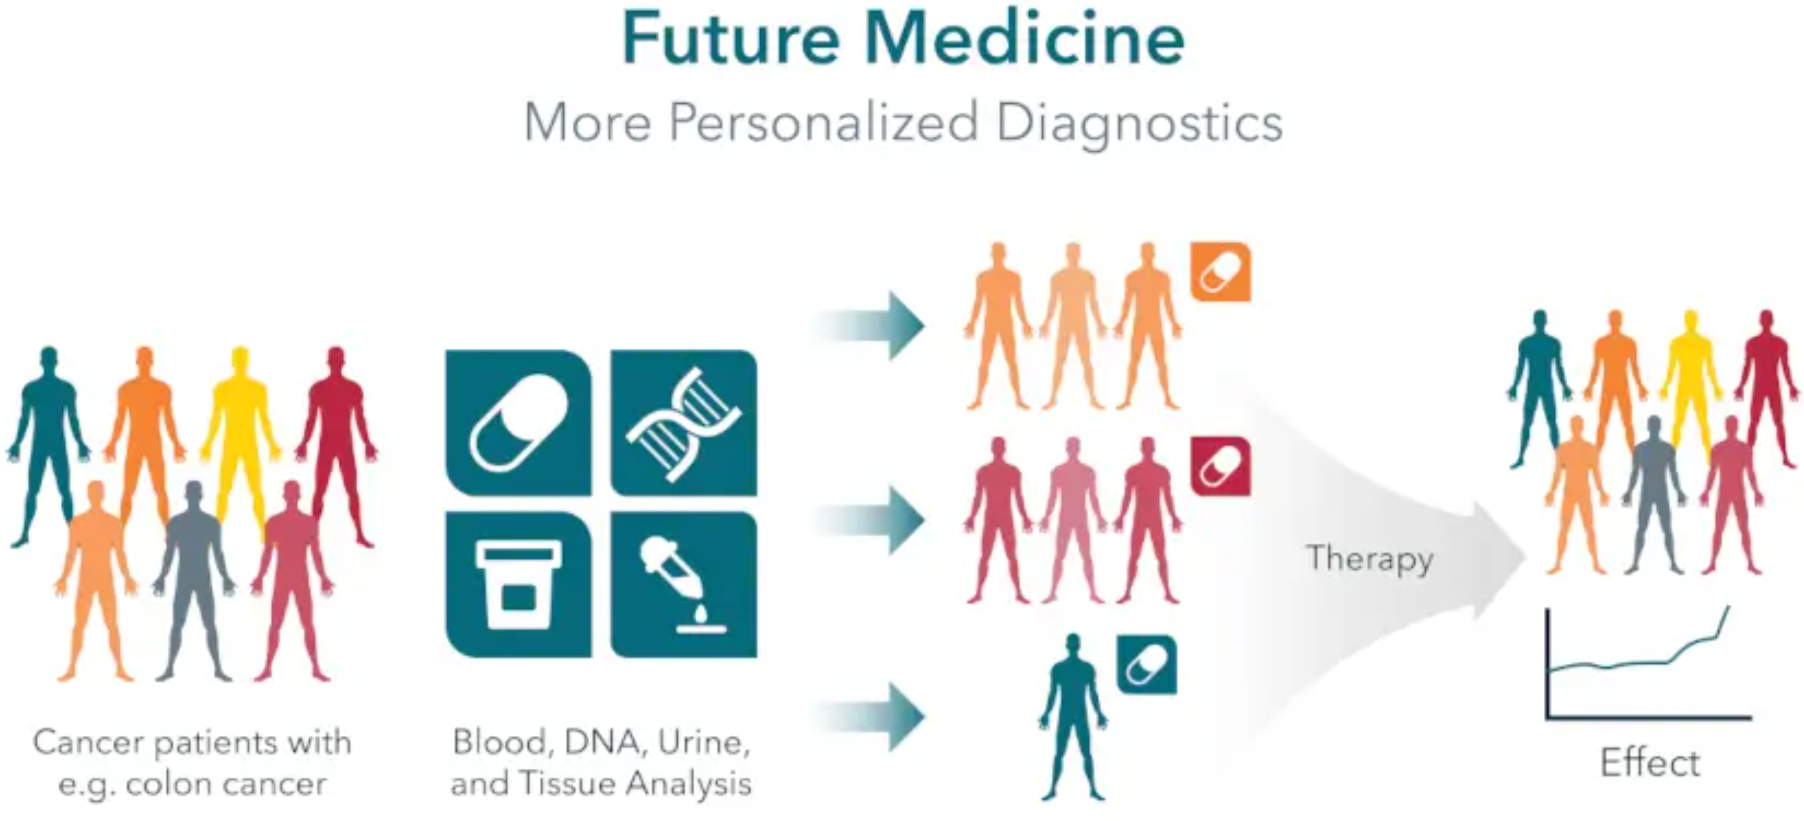
\includegraphics[width=\textwidth]{../img/introduction/medecine_future}
		\caption{Cada paciente necesita un tratamiento personalizado. \textbf{Fuente} The Atlas Cancer \cite{pdx2023}.}
	\end{figure}
\end{frame}
%-------------------------------------------------------
%-------------------------------------------------------












%-------------------------------------------------------
%-------------------------------------------------------
\begin{frame}{Inmunoterapia del Cáncer}{}		
	Es un tipo de tratamiento contra el Cáncer que estimula las defensas naturales del cuerpo para combatir el Cáncer \cite{inmunoterapy2022}.
		
	\begin{figure}
		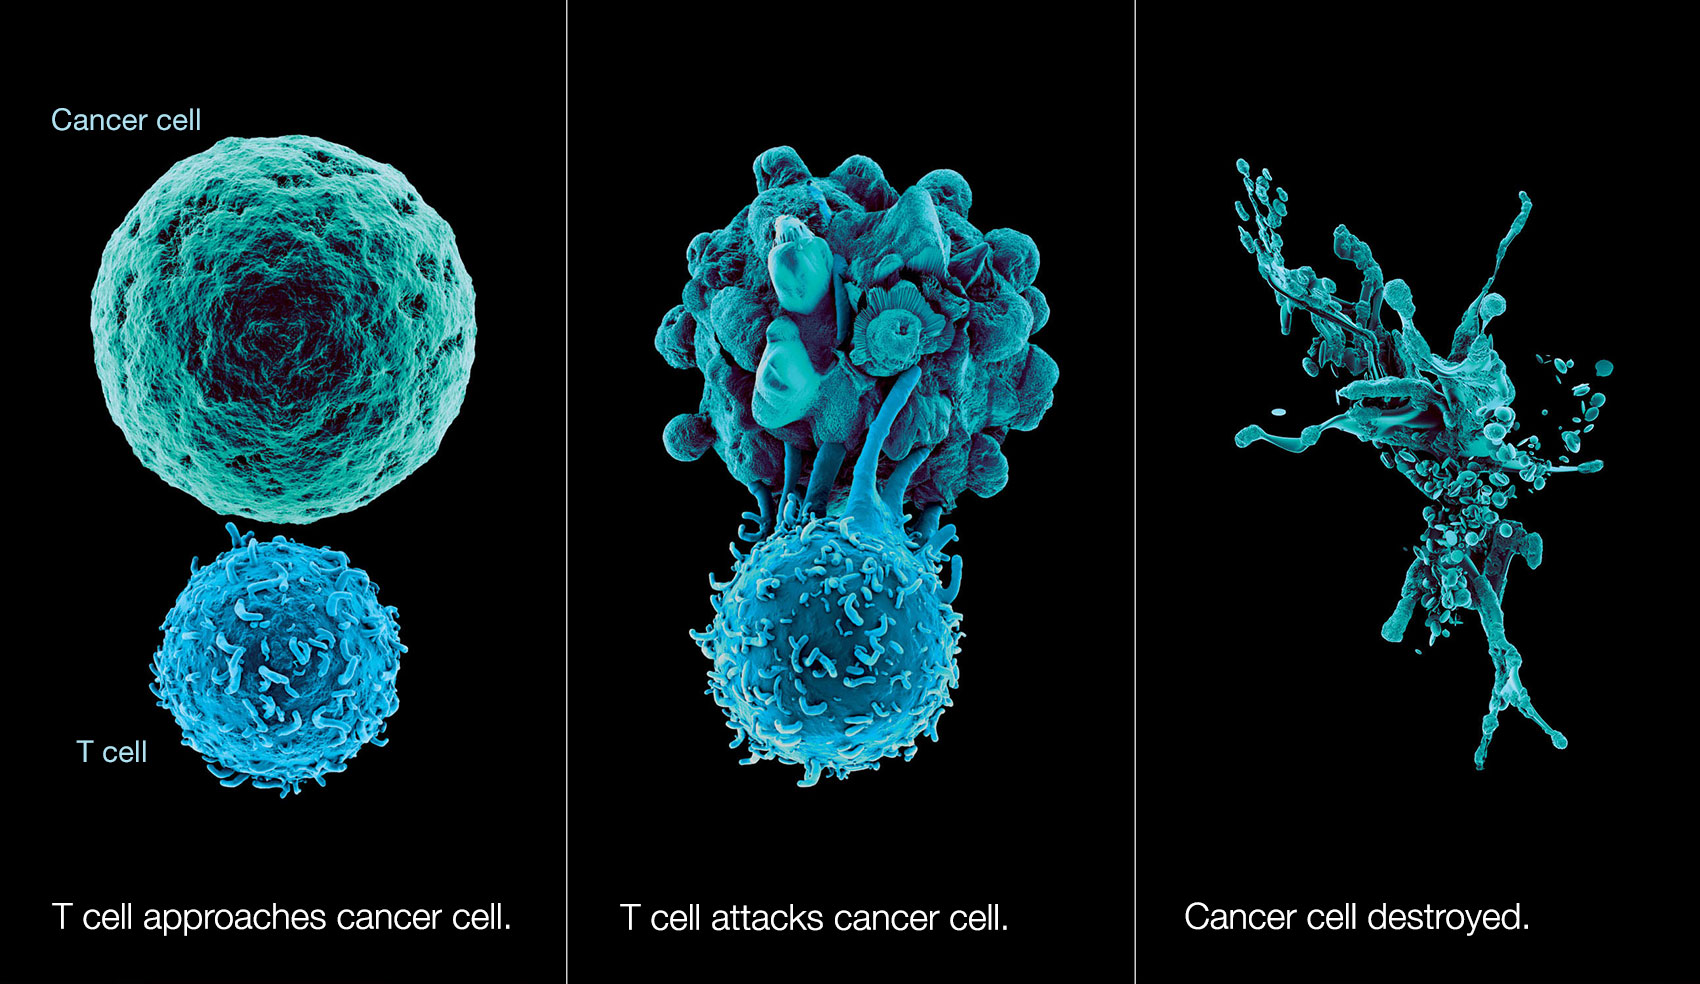
\includegraphics[width=0.85\textwidth]{../img/neoantigen/tcell}
		\caption{Ejemplo de como una célula T destruye células del cancer \cite{nortshore2022}.}
	\end{figure}		
\end{frame}
%-------------------------------------------------------
%-------------------------------------------------------


%-------------------------------------------------------
%-------------------------------------------------------
\begin{frame}{Contexto y Motivación}{Inmunoterapia del Cáncer}
	
	
	\begin{figure}[]
		\centering
		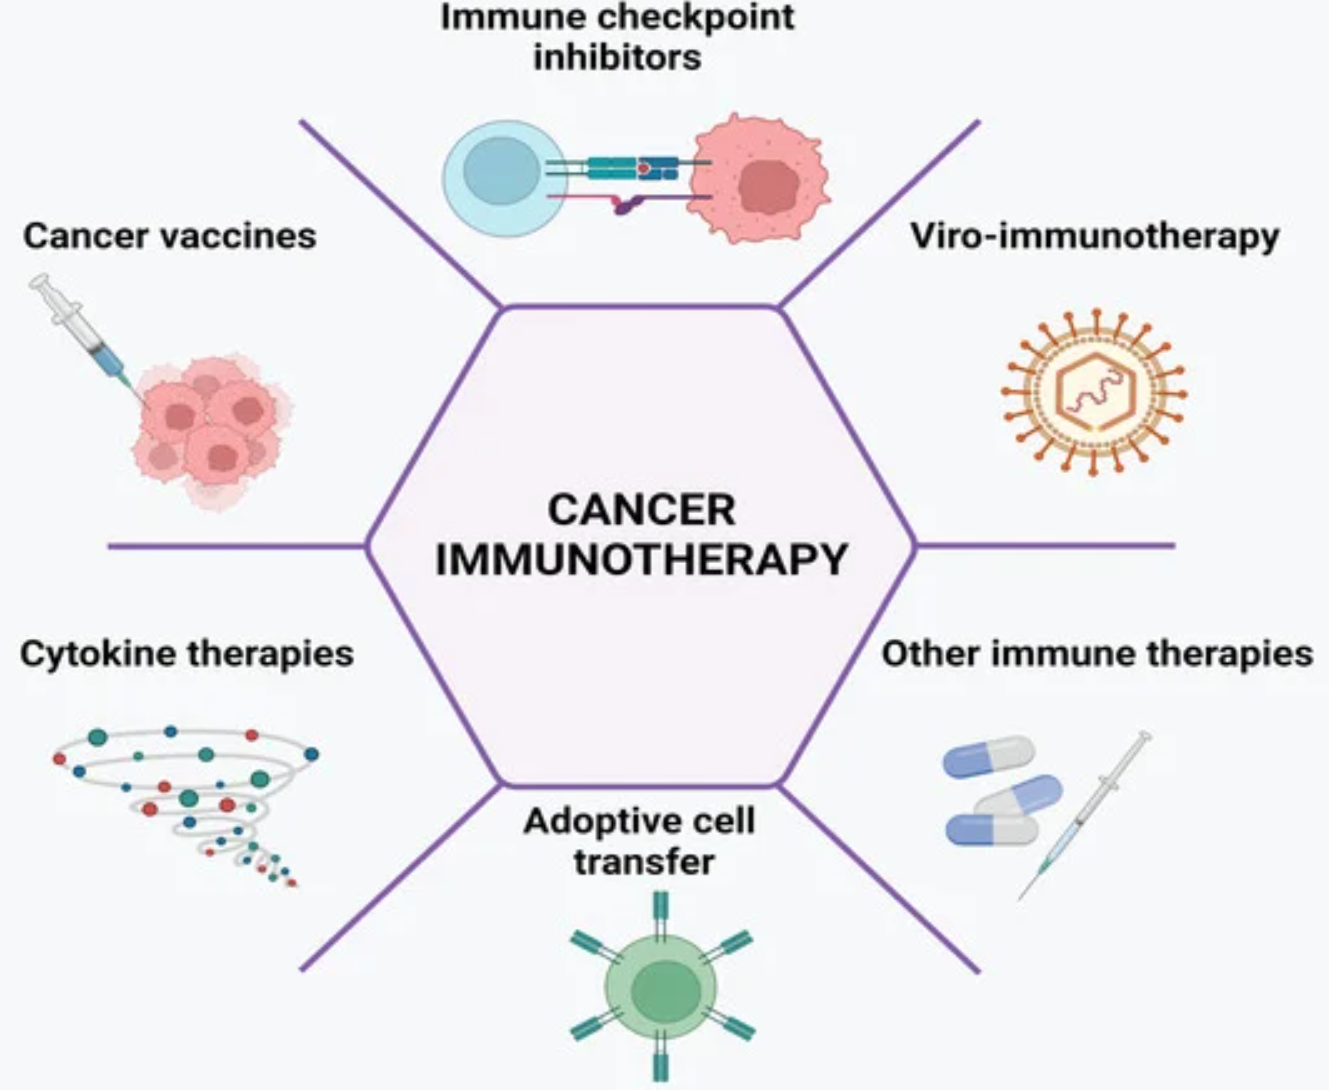
\includegraphics[width=0.7\textwidth]{../img/introduction/cancer_immunotherapy}
		\caption{Tipos de tratamientos para la inmunoterapia del cáncer. \textbf{Fuente}: \cite{kciuk2023recent}.}
	\end{figure}
\end{frame}
%-------------------------------------------------------
%-------------------------------------------------------


%%%%%%%%%%%%%%%%%%%%%%%%%%%%%%%%%%%%%%%%%%%%%%%%%%%%%%%%%%%%%%%%%%%%%%%%%%%%%%%%%%%%%%%%%%%%%%%%%%%%%%%%%%%%%%%%
\subsection{Vacunas Personalizadas}
%%%%%%%%%%%%%%%%%%%%%%%%%%%%%%%%%%%%%%%%%%%%%%%%%%%%%%%%%%%%%%%%%%%%%%%%%%%%%%%%%%%%%%%%%%%%%%%%%%%%%%%%%%%%%%%%




%-------------------------------------------------------
%-------------------------------------------------------
\begin{frame}{Contexto y Motivación}{Neoantígenos}
	Es una \textbf{proteína} que se forma en las células de Cáncer cuando ocurre mutaciones en el DNA  \cite{NCIdictionary2022, borden2022cancer}.
	
	\begin{figure}[]
		\centering
		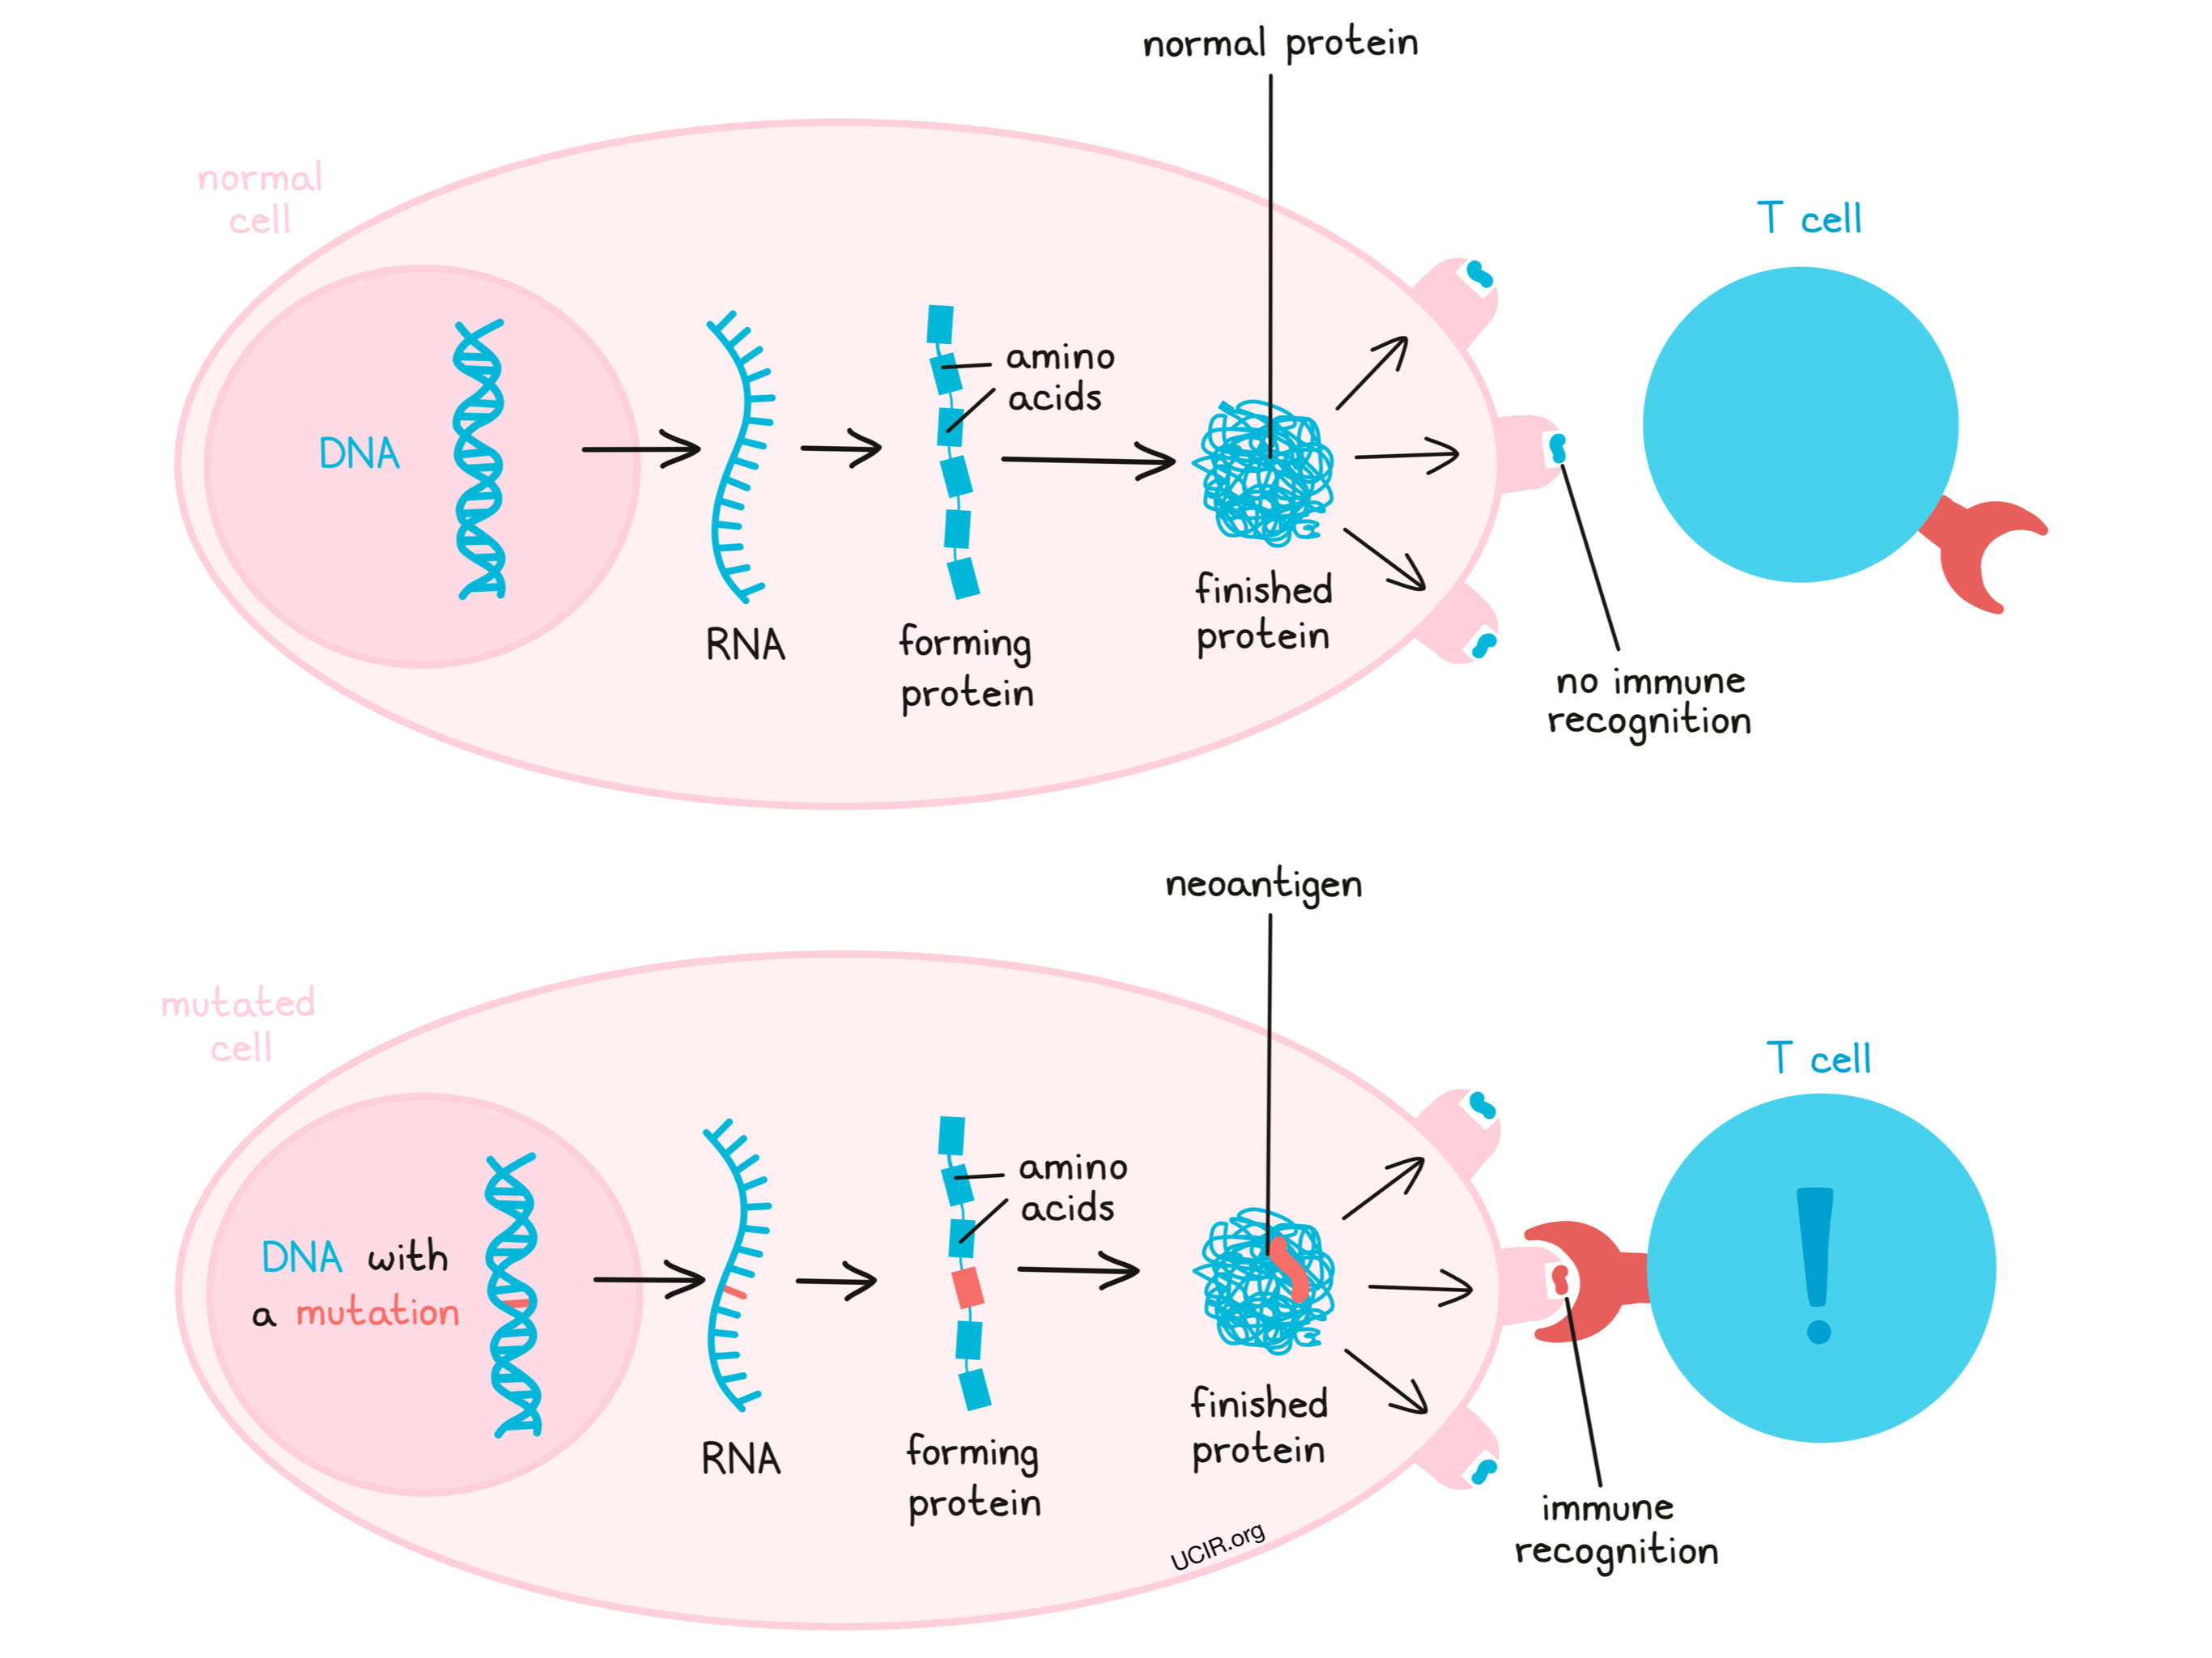
\includegraphics[width=0.7\textwidth]{../img/introduction/neoantigen}
		\caption{Neoantígenos y células T. \textbf{Fuente}: \cite{ucir2023}.}
	\end{figure}
\end{frame}
%-------------------------------------------------------
%-------------------------------------------------------

%-------------------------------------------------------
%-------------------------------------------------------
\begin{frame}{Contexto y Motivación}{Vacunas personalizadas}	
	\begin{figure}[H]
		\centering
		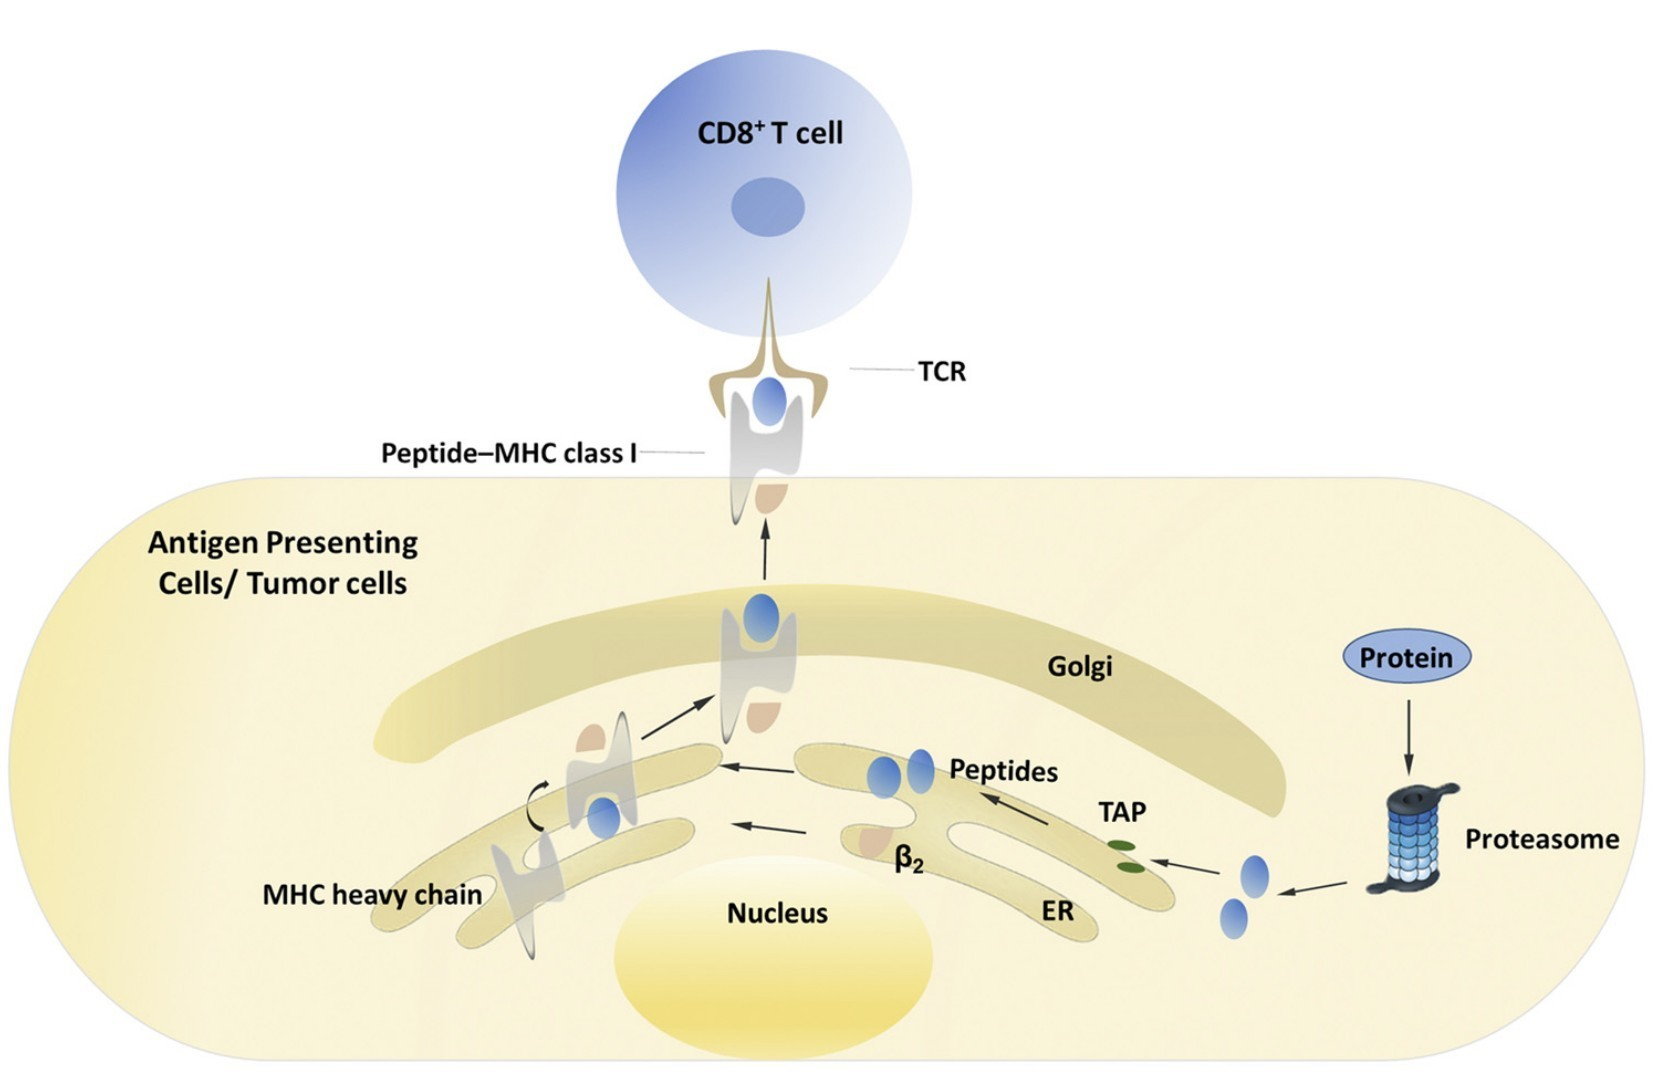
\includegraphics[width=0.9\textwidth]{../img/neoantigen/mhc1.jpg}
		\caption{Presentación de antígenos por MHC-I. Fuente: \cite{zhang2019application}}
		\label{fig:mhc1}
	\end{figure}	
\end{frame}
%-------------------------------------------------------
%-------------------------------------------------------

%%-------------------------------------------------------
%%-------------------------------------------------------
%\begin{frame}{MHC-II}{}		%
%	\begin{figure}[H]
	%		\centering
	%		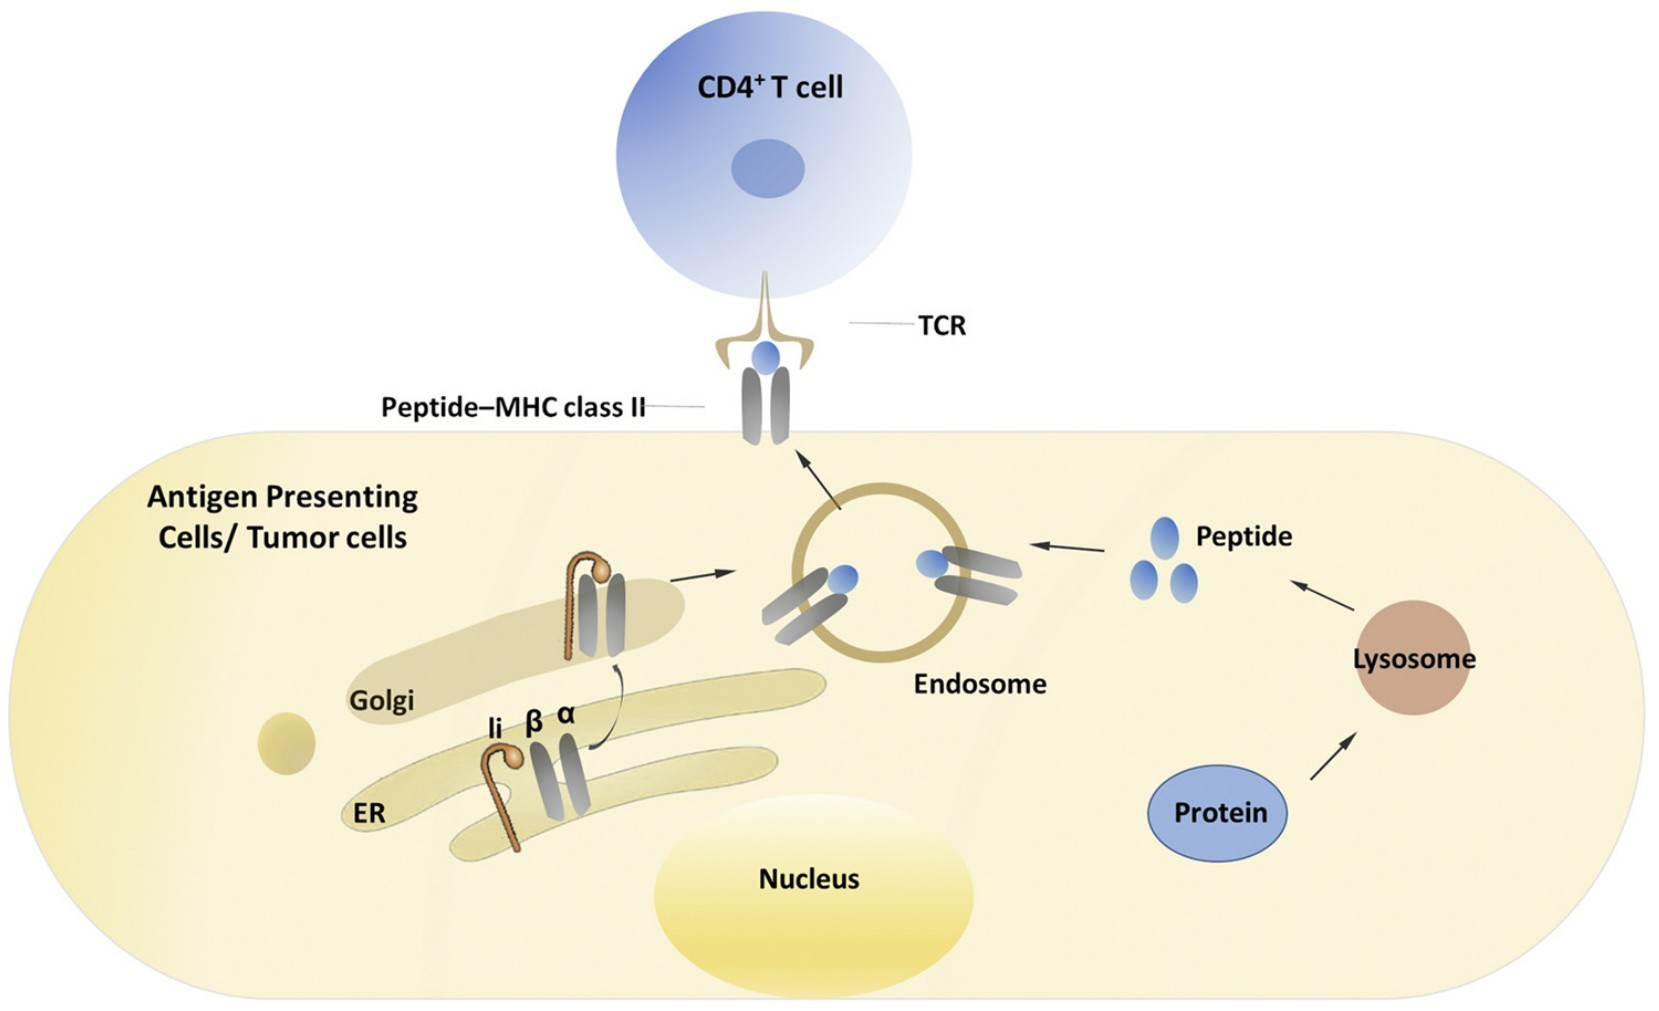
\includegraphics[width=0.9\textwidth]{../img/neoantigen/mhc2.jpg}
	%		\caption{Presentación de antígenos por MHC-II. Fuente: \cite{zhang2019application}}
	%		\label{fig:mhc2}
	%	\end{figure}	
%\end{frame}
%-------------------------------------------------------
%-------------------------------------------------------

%-------------------------------------------------------
%-------------------------------------------------------
\begin{frame}{Contexto y Motivación}{Vacunas personalizadas}	
	\begin{figure}[]
		\centering
		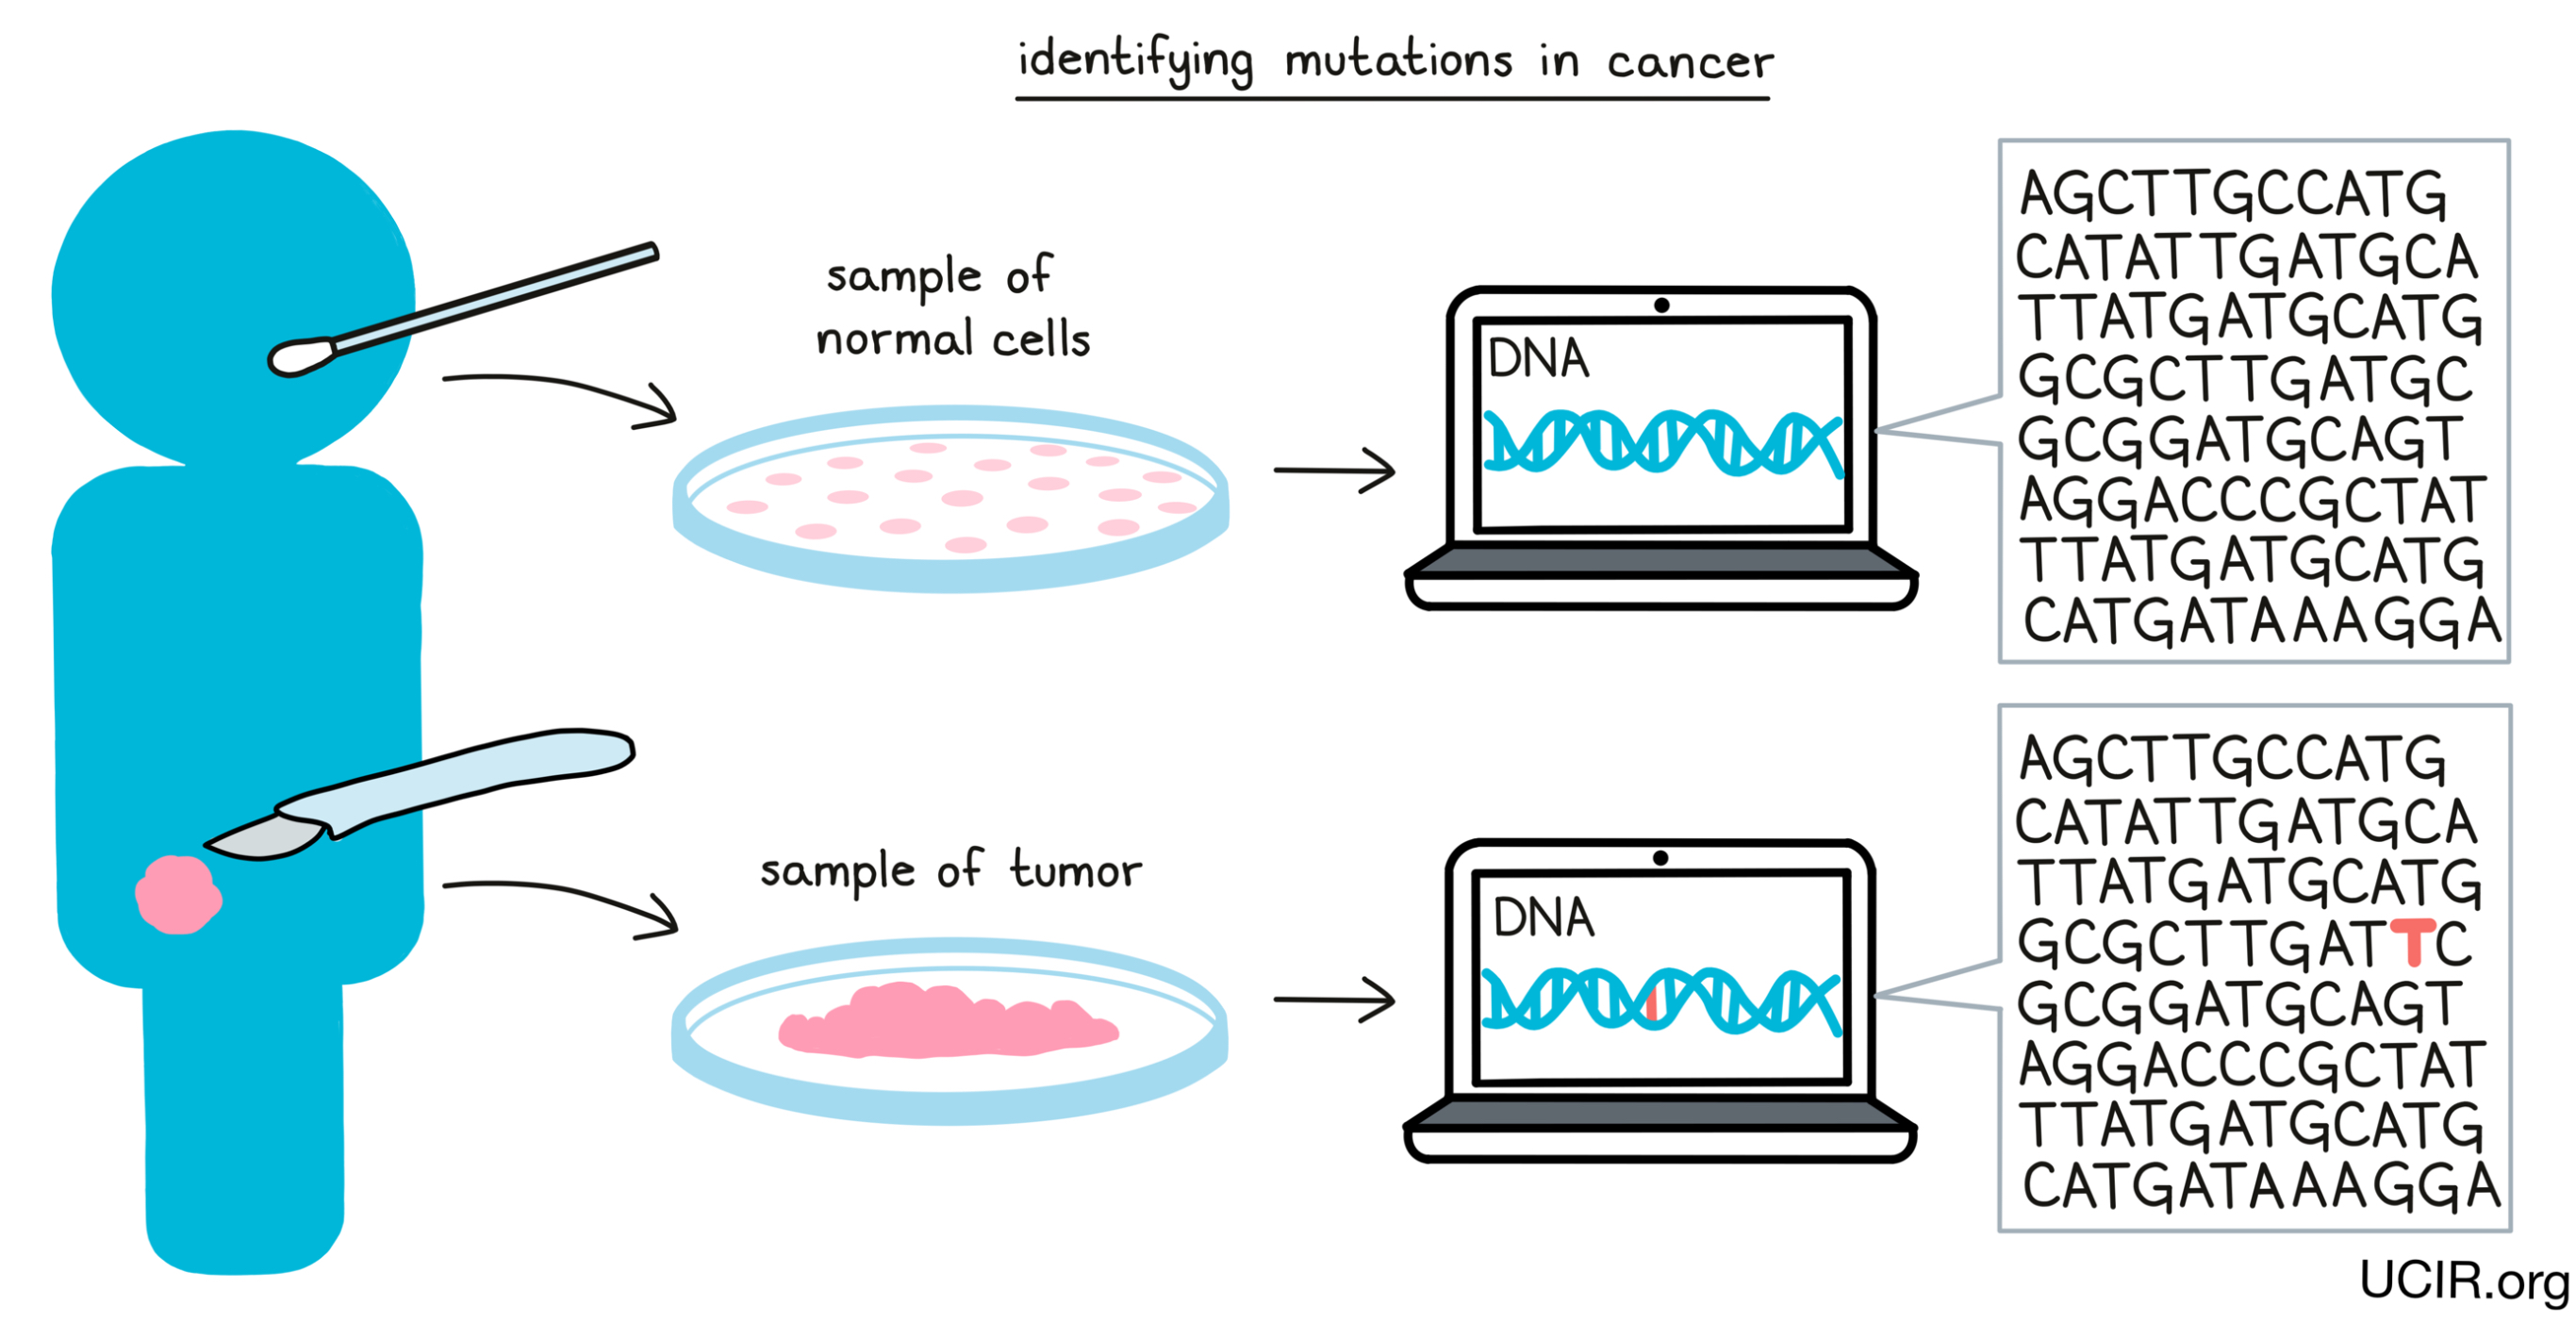
\includegraphics[width=\textwidth]{../img/introduction/vaccine_1}
		\caption{Proceso para la generación de vacunas contra el cáncer. \textbf{Fuente}: \cite{ucir2023}.}
	\end{figure}
\end{frame}
%-------------------------------------------------------
%-------------------------------------------------------



%-------------------------------------------------------
%-------------------------------------------------------
\begin{frame}{Contexto y Motivación}{Vacunas personalizadas}	
	\begin{figure}[]
		\centering
		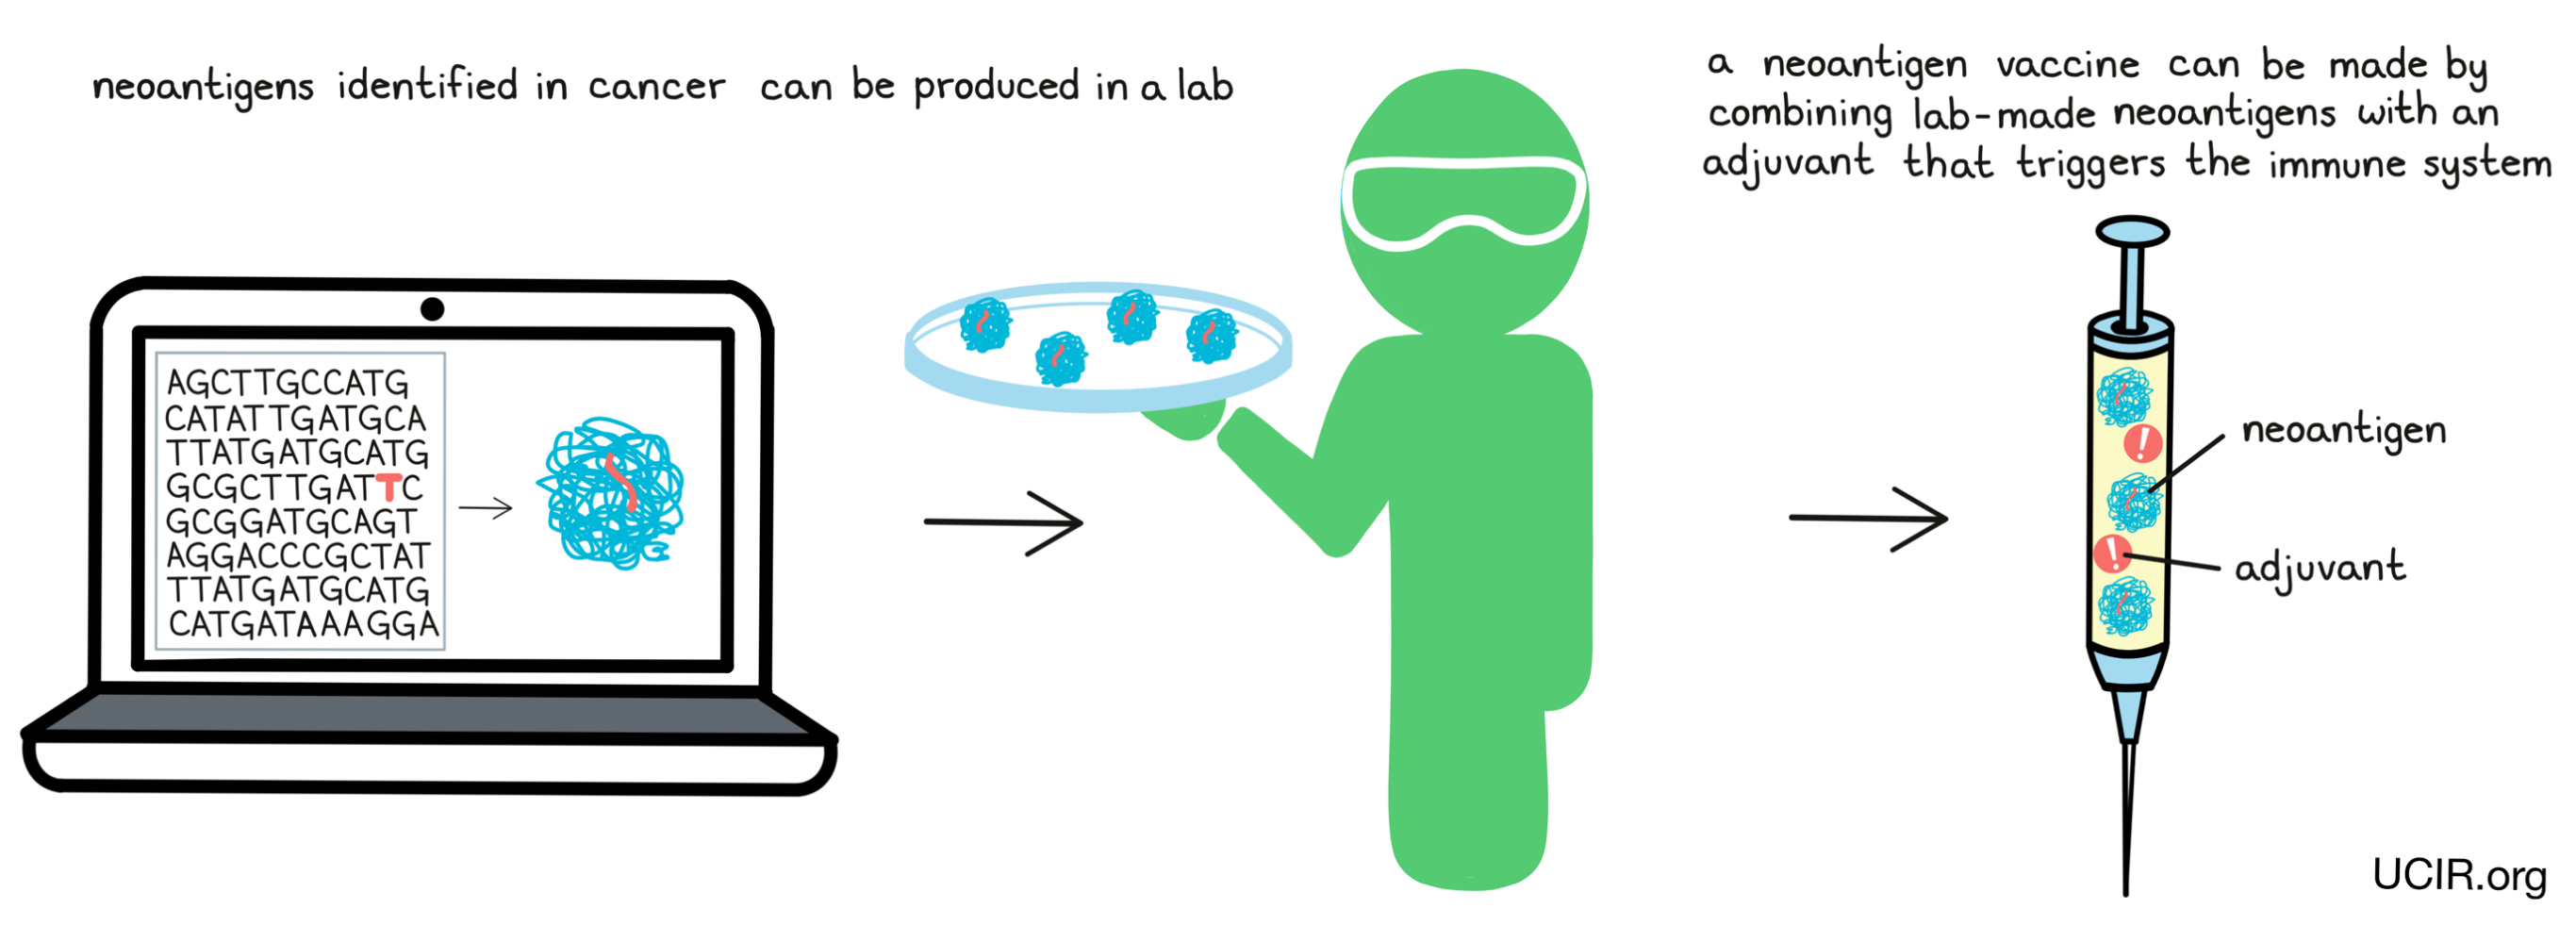
\includegraphics[width=\textwidth]{../img/introduction/vaccine_2}
		\caption{Proceso para la generación de vacunas contra el cáncer. \textbf{Fuente}: \cite{ucir2023}.}
	\end{figure}
\end{frame}
%-------------------------------------------------------
%-------------------------------------------------------

%-------------------------------------------------------
%-------------------------------------------------------
\begin{frame}{Contexto y Motivación}{Vacunas personalizadas}	
	\begin{figure}[]
		\centering
		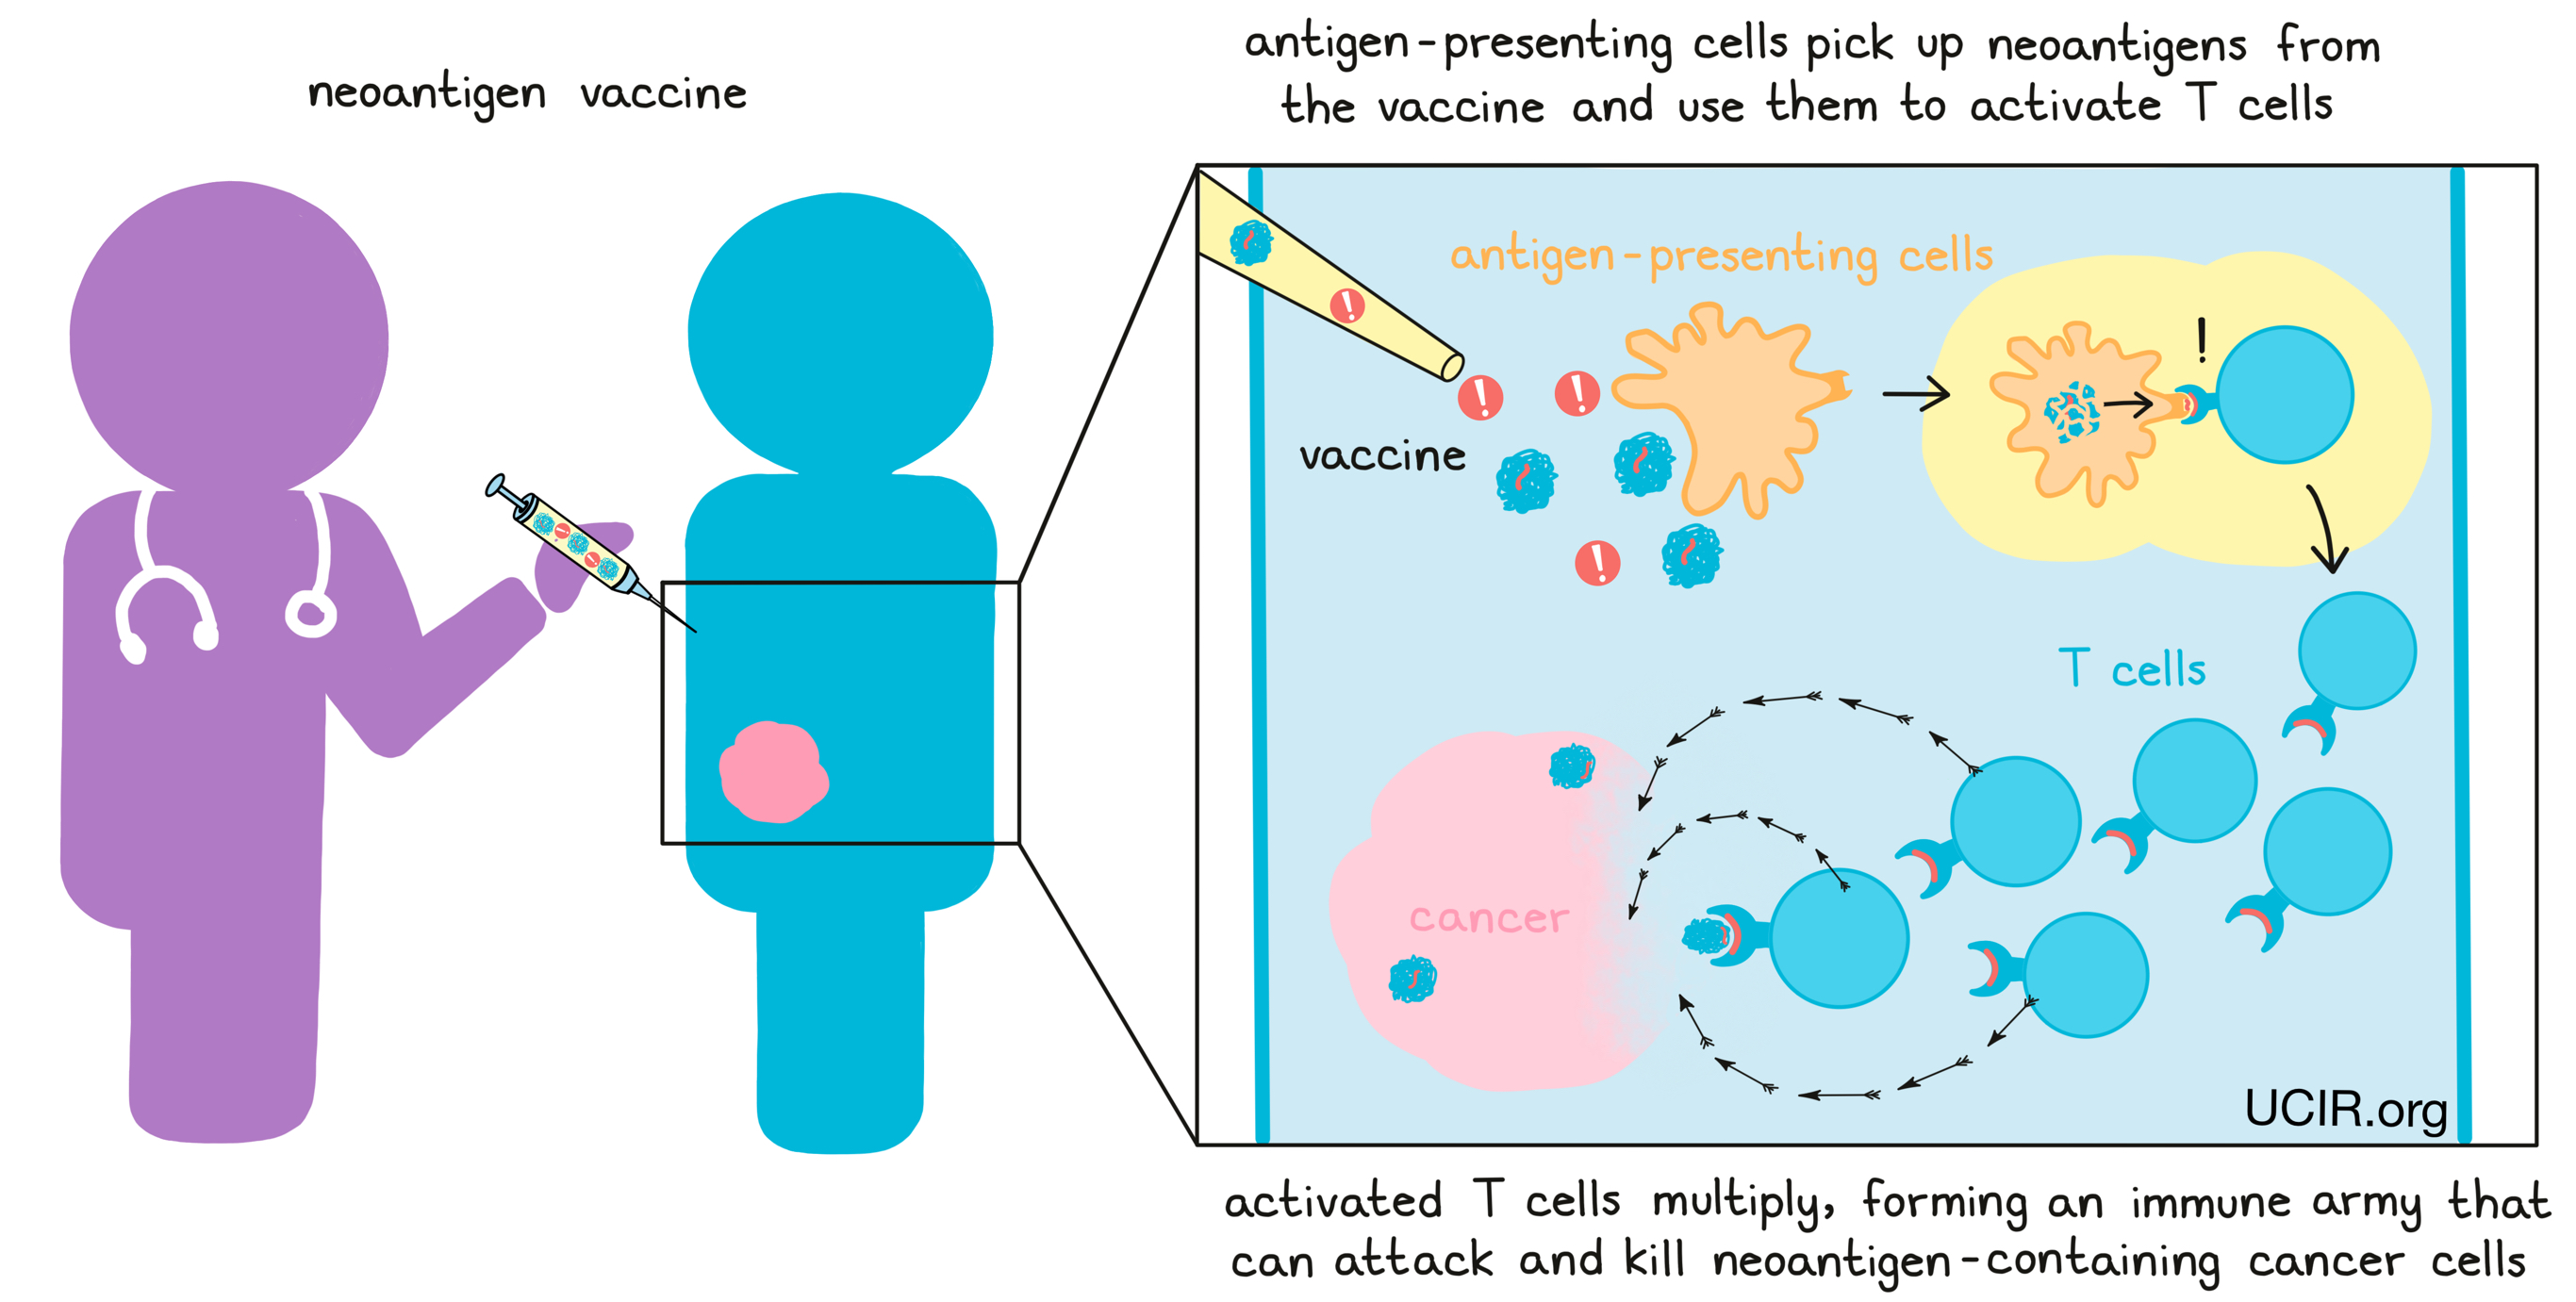
\includegraphics[width=\textwidth]{../img/introduction/vaccine_3}
		\caption{Proceso para la generación de vacunas contra el cáncer. \textbf{Fuente}: \cite{ucir2023}.}
	\end{figure}
\end{frame}
%-------------------------------------------------------
%-------------------------------------------------------

	%-------------------------------------------------------
%-------------------------------------------------------
\begin{frame}{Contexto y Motivación}{Vacunas personalizadas}
	\begin{figure}
		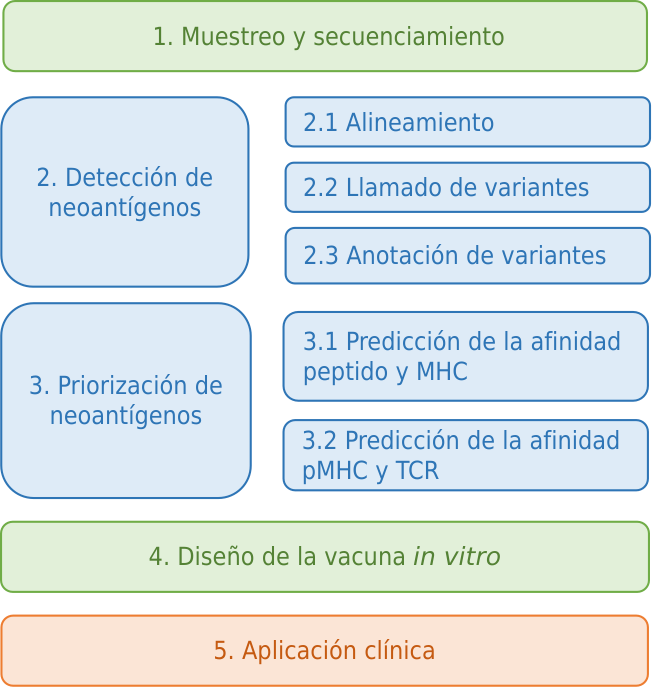
\includegraphics[width=0.5\textwidth]{../img/pipeline/pipeline_spanish}
		\caption{Resumen del proceso de  generación de vacunas contra el cáncer.}
	\end{figure}		
\end{frame}
%-------------------------------------------------------
%-------------------------------------------------------


%%%%%%%%%%%%%%%%%%%%%%%%%%%%%%%%%%%%%%%%%%%%%%%%%%%%%%%%%%%%%%%%%%%%%%%%%%%%%%%%%%%%%%%%%%%%%%%%%%%%%%%%%%%%%%%%
%%%%%%%%%%%%%%%%%%%%%%%%%%%%%%%%%%%%%%%%%%%%%%%%%%%%%%%%%%%%%%%%%%%%%%%%%%%%%%%%%%%%%%%%%%%%%%%%%%%%%%%%%%%%%%%%
%%%%%%%%%%%%%%%%%%%%%%%%%%%%%%%%%%%%%%%%%%%%%%%%%%%%%%%%%%%%%%%%%%%%%%%%%%%%%%%%%%%%%%%%%%%%%%%%%%%%%%%%%%%%%%%%
\section{Problema y Objetivos}
%%%%%%%%%%%%%%%%%%%%%%%%%%%%%%%%%%%%%%%%%%%%%%%%%%%%%%%%%%%%%%%%%%%%%%%%%%%%%%%%%%%%%%%%%%%%%%%%%%%%%%%%%%%%%%%%
%%%%%%%%%%%%%%%%%%%%%%%%%%%%%%%%%%%%%%%%%%%%%%%%%%%%%%%%%%%%%%%%%%%%%%%%%%%%%%%%%%%%%%%%%%%%%%%%%%%%%%%%%%%%%%%%
%%%%%%%%%%%%%%%%%%%%%%%%%%%%%%%%%%%%%%%%%%%%%%%%%%%%%%%%%%%%%%%%%%%%%%%%%%%%%%%%%%%%%%%%%%%%%%%%%%%%%%%%%%%%%%%%

\subsection{Motivación y Problema}

%-------------------------------------------------------
%-------------------------------------------------------
\begin{frame}{Motivación}{}	

\begin{block}{}
	El cáncer representa el mayor problema de salud mundial, pero lamentablemente los métodos basados en cirugías, radioterapias, quimioterapias tienen baja efectividad \cite{peng2019neoantigen}.
\end{block}	

\begin{block}{}
	La inmunoterapia del cáncer es una alternativa para el desarrollo de vacunas personalizadas, pero este proceso depende de una correcta detección de neo antígenos \cite{de2020neoantigen, peng2019neoantigen}.
\end{block}

\end{frame}
%-------------------------------------------------------
%-------------------------------------------------------



%-------------------------------------------------------
%-------------------------------------------------------
\begin{frame}{Problema}{}
	
\begin{block}{}
	Menos del \textbf{5\% de péptidos} detectados en \textit{pMHC binding}, llegan a la membrana de la células.  Para \textit{peptide-MHC presentation}, propuestas recientes solo llegan a \textbf{0.6 de \textit{presicion} y 0.4 de \textit{recall}} \cite{mill2022neoms}. 
\end{block}
	


\begin{block}{}
	En este contexto, la tesis se enfoca en el problema de \textit{pMHC presentation}, considerándolo como un problema de clasificación binaria, y tomando como entrada la secuencia de aminoácidos del péptido y la secuencia de aminoácidos de la proteína MHC. 
\end{block}
	
\end{frame}
%-------------------------------------------------------
%-------------------------------------------------------

\subsection{Objetivo}

%-------------------------------------------------------
%-------------------------------------------------------
\begin{frame}{Objetivos}{Objetivo general}	
	\begin{block}{Objetivo general}
		Proponer un método basado en \textit{deep learning} para la detección de neo antígenos, enfocados en el problema de \textit{peptide-MHC presentation}.  
	\end{block}	
\end{frame}
%-------------------------------------------------------
%-------------------------------------------------------

%-------------------------------------------------------
%-------------------------------------------------------
%\begin{frame}{Objetivos}{}	
%	\begin{figure}
%		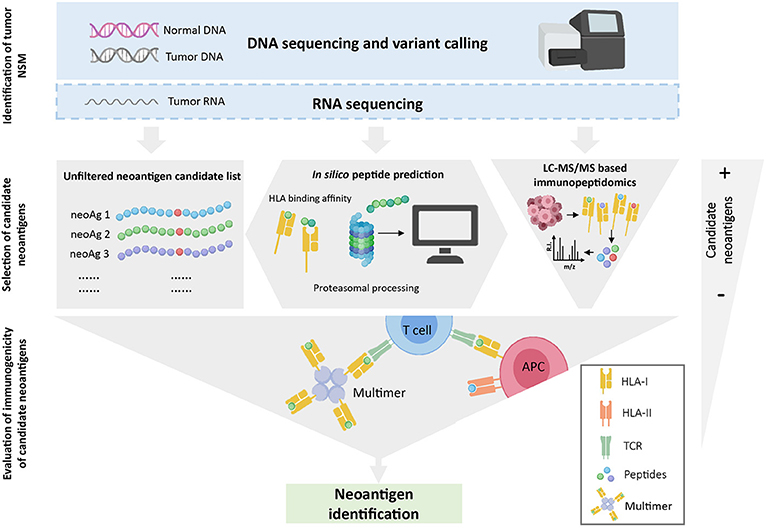
\includegraphics[width=0.97\textwidth]{img/neoantigen/pipeline_neoantigen}
		%\caption{Proceso de la detección de neo antígenos \cite{garcia2019determinants}.}
%	\end{figure}
%\end{frame}
%-------------------------------------------------------
%-------------------------------------------------------


%%%%%%%%%%%%%%%%%%%%%%%%%%%%%%%%%%%%%%%%%%%%%%%%%%%%%%%%%%%%%%%%%%%%%%%%%%%%%%%%%%%%%%%%%%%%%%%%%%%%%%%%%%%%%%%%
%%%%%%%%%%%%%%%%%%%%%%%%%%%%%%%%%%%%%%%%%%%%%%%%%%%%%%%%%%%%%%%%%%%%%%%%%%%%%%%%%%%%%%
\section{Revisión Sistemática de la Literatura (RSL)}
%%%%%%%%%%%%%%%%%%%%%%%%%%%%%%%%%%%%%%%%%%%%%%%%%%%%%%%%%%%%%%%%%%%%%%%%%%%%%%%%%%%%%%%%%%%%%%%%%%%%%%%%%%%%%%%%
%%%%%%%%%%%%%%%%%%%%%%%%%%%%%%%%%%%%%%%%%%%%%%%%%%%%%%%%%%%%%%%%%%%%%%%%%%%%%%%%%%%%%%

%%%%%%%%%%%%%%%%%%%%%%%%%%%%%%%%%%%%%%%%%%%%%%%%%%%%%%%%%%%%%%%%%%%%%%%%%%%%%%%%%%%%%%%%%%%%%%%%%%%%%%%%%%%%%%%%
%%%%%%%%%%%%%%%%%%%%%%%%%%%%%%%%%%%%%%%%%%%%%%%%%%%%%%%%%%%%%%%%%%%%%%%%%%%%%%%%%%%%%%
\subsection{Metodología}
%%%%%%%%%%%%%%%%%%%%%%%%%%%%%%%%%%%%%%%%%%%%%%%%%%%%%%%%%%%%%%%%%%%%%%%%%%%%%%%%%%%%%%%%%%%%%%%%%%%%%%%%%%%%%%%%
%%%%%%%%%%%%%%%%%%%%%%%%%%%%%%%%%%%%%%%%%%%%%%%%%%%%%%%%%%%%%%%%%%%%%%%%%%%%%%%%%%%%%%


%-------------------------------------------------------
%-------------------------------------------------------
\begin{frame}{RSL}{Metodología}

	\begin{table}[H]
		\begin{center}
			\caption{Cadenas de busqueda utilizadas en la RSL.}
			\label{tab:key_words}
			\setlength{\tabcolsep}{0.5em} % for the horizontal padding
			{\renewcommand{\arraystretch}{1.4}% for the vertical padding
				\begin{tabular}{p{10cm}}
					\textbf{Cadena de busqueda} \\ \hline
					neoantigen  AND (detection OR pipeline) AND deep learning                                                                               \\
					(MHC OR HLA) AND binding  AND deep learning                                                                                             \\				
					(MHC-I OR MHC-II OR MHC OR HLA) AND (peptide OR epitope) AND ( binding OR affinity OR prediction OR detection OR presentation)          \\
					TCR interaction prediction                                                                                                              \\		
				\end{tabular}
			}
		\end{center}
	\end{table}
\end{frame}
%-------------------------------------------------------
%-------------------------------------------------------


%-------------------------------------------------------
%-------------------------------------------------------
\begin{frame}{RSL}{Metodología}
	
	\begin{table}[H]
		\centering
		\begin{center}
			\caption{Bases de datos utilizadas en la RSL.}
			\label{tab:bd_RSL}
			\setlength{\tabcolsep}{0.5em} % for the horizontal padding
			{\renewcommand{\arraystretch}{1.2}% for the vertical padding
				\begin{tabular}{p{3cm}}
					\textbf{Bases de datos} \\ \hline
					IEEE Xplore                                                                               \\
					Science Direct \\				
					Springer          \\
					ACM Digital Library                                                                                                             \\	
					PubMed \\ 
					BioRxiv \\ 	
				\end{tabular}
			}
		\end{center}
	\end{table}

\end{frame}
%-------------------------------------------------------
%-------------------------------------------------------



%-------------------------------------------------------
%-------------------------------------------------------
\begin{frame}{RSL}{Metodología}
	
\begin{table}[H]
	\begin{center}
		\caption{Criterios de inclusión y exclusión de artículos utilizados en la RSL.}
		\label{tab:criterios}
		\setlength{\tabcolsep}{0.5em} % for the horizontal padding
		{\renewcommand{\arraystretch}{1.2}% for the vertical padding
			\begin{tabular}{p{5cm}p{5cm}}
				\textbf{Criterios de inclusión}                                                   & \textbf{Criterios de exclusión}                                                           \\ \hline
				Artículos con categoría ERA (A, B o C) si son conferencias y Journals Q1, Q2 o Q3. & Trabajos de baja calidad, que no esten rankeados.                                      \\
				Sobre \textit{deep learning}                \\
				La metodología es detallada.                                                                                                               &                                                                                                        \\
				Tiene repositorio de código fuente y base de datos (deseable).                                          &                                                                                                        \\
				                                                                                                       
			\end{tabular}
		}
	\end{center}
\end{table}
	
\end{frame}
%-------------------------------------------------------
%-------------------------------------------------------






%-------------------------------------------------------
%-------------------------------------------------------
\begin{frame}{RSL}{Metodología}
	
	\begin{table}[H]
		\begin{center}
			\caption{Cantidad de artículos encontrados y seleccionados según los criterios de inclusión y exclusión en la RSL.}
			\label{tab:number_papers}
			\setlength{\tabcolsep}{0.5em} % for the horizontal padding
			{\renewcommand{\arraystretch}{1.2}% for the vertical padding
				\begin{tabular}{ccc}
					\textbf{Año} & \textbf{Artículos encontrados} & \textbf{Artículos seleccionados}\\ \hline
					2018 & 57 & 21 \\
					2019 & 72 & 31 \\
					2020 & 86 & 29 \\
					2021 & 61 & 34 \\
					2022 & 58 & 19 \\ \hline
					Total & \textbf{334} & \textbf{134} \\
				\end{tabular}
			}
		\end{center}
	\end{table}
	
\end{frame}
%-------------------------------------------------------
%-------------------------------------------------------

%%%%%%%%%%%%%%%%%%%%%%%%%%%%%%%%%%%%%%%%%%%%%%%%%%%%%%%%%%%%%%%%%%%%%%%%%%%%%%%%%%%%%%%%%%%%%%%%%%%%%%%%%%%%%%%%
%%%%%%%%%%%%%%%%%%%%%%%%%%%%%%%%%%%%%%%%%%%%%%%%%%%%%%%%%%%%%%%%%%%%%%%%%%%%%%%%%%%%%%
\subsection{Resultados}
%%%%%%%%%%%%%%%%%%%%%%%%%%%%%%%%%%%%%%%%%%%%%%%%%%%%%%%%%%%%%%%%%%%%%%%%%%%%%%%%%%%%%%%%%%%%%%%%%%%%%%%%%%%%%%%%
%%%%%%%%%%%%%%%%%%%%%%%%%%%%%%%%%%%%%%%%%%%%%%%%%%%%%%%%%%%%%%%%%%%%%%%%%%%%%%%%%%%%%%
%-------------------------------------------------------
%-------------------------------------------------------
\begin{frame}{RSL}{Convolutional Neural Networks}
	
	\fontsize{8pt}{5pt}\selectfont
	
	\begin{table}[]
		\centering
		\caption{List of research since 2018 that uses CNNs for peptide-MHC binding and presentation.}
		\setlength{\tabcolsep}{0.5em} % for the horizontal padding
		{\renewcommand{\arraystretch}{2}% for the vertical padding
			\begin{tabular}{p{0.6cm}p{0.6cm}p{1.5cm}p{2cm}p{0.6cm}p{2.7cm}}
				\textbf{Year} & \textbf{Ref.}                              & \textbf{Approach}        & \textbf{Name} & \textbf{MHC} & \textbf{Encoding}                                                                                                                                                                                   \\ \hline
				
				2022 &	\cite{you2022deepmhcii}	& pMHC(b) &	DeepMHCII &	 II &	PFR \\
				
				2021          & \cite{li2021deepimmuno}   & pMHC(b)      & DeepImmuno    &  I        & AAindex1                                                \\
				2021          & \cite{lang2021neofox}     & pMHC(p) & APPM          &  I        & One-hot                                                                          \\
				2021          & \cite{lee2021connecting}  & pMHC(p) & MHCfovea      &  I        & One-hot                                                                                                      \\
				2021          & \cite{junet2021cnn}       & pMHC(b)      & CNN-PepPred   &  II       & BLOSUM     \\
				
				2020          & \cite{pei2020iconmhc}     & pMHC(b)      & IConMHC       & I        & PCA and AAindex3        \\
				2020          & \cite{saxena2020onionmhc} & pMHC(b)      & OnionMHC      & I        & BLOSUM and structural features                                                                  \\
				2020          & \cite{ng3704016minerva}   & pMHC(p) & MINERVA       & I        & Physicochemical properties                                                           \\
				2019          & \cite{zhao2019peptide}    & pMHC(b)      & CNN-NF        & I        & Sequence, Hydropathy, Polarity, Length                    \\
				2019          & \cite{liu2019deepseqpan}  & pMHC(b)      & DeepSeqPan    & I        & One-hot                                          \\
				2018          & \cite{han2018deep}        & pMHC(b)      & ConvMHC       & I        & Contact side HLA.peptide                                                                                 
			\end{tabular}
		}
		\end{table}	
\end{frame}
%-------------------------------------------------------
%-------------------------------------------------------


%-------------------------------------------------------
%-------------------------------------------------------
\begin{frame}{RSL}{Convolutional Neural Networks}
	
	\fontsize{8pt}{5pt}\selectfont
	
	\begin{table}[]
		\centering
		\caption{List of research since 2018 that uses CNNs s with RNN or attention mechanisms for peptide-MHC binding and presentation. MHCherryPan uses CNN with RNN, the other uses CNN witn Attention mechanims.}		
		\setlength{\tabcolsep}{0.5em} % for the horizontal padding
		{\renewcommand{\arraystretch}{2}% for the vertical padding
			\begin{tabular}{p{0.6cm}p{0.6cm}p{1.5cm}p{2cm}p{0.6cm}p{2.7cm}}
			\textbf{Year} & \textbf{Ref.}                              & \textbf{Approach}   & \textbf{Name}    & \textbf{MHC} & \textbf{Encoding}                                           \\ \hline
			2021          & \cite{yang2021deepnetbim} & pMHC(b) & DeepNetBim       & I        & BLOSUM              \\
			
			2021          & \cite{jin2021deep}        & pMHC(b) & Deep Attention Pan & I        & BLOSUM                    \\
			
			2019          & \cite{hu2019acme}         & pMHC(b) & ACME             & I        & BLOSUM      \\
			
			2020          & \cite{xie2020mhcherrypan} & pMHC(b) & MHCherryPan      & I        & BLOSUM          
		\end{tabular}
		}
	\end{table}	
\end{frame}
%-------------------------------------------------------
%-------------------------------------------------------


%-------------------------------------------------------
%-------------------------------------------------------
\begin{frame}{RSL}{Recurrent Neural Networks}
	
	\fontsize{8pt}{5pt}\selectfont
	
	\begin{table}[]
		\centering
		\caption{List of research since 2018 that uses RNNs for peptide-MHC binding and presentation. MATHLA, DeepSeqPanII and DeepHLApan uses RNN with attention mechanims, meanwhile the other focus on GRU and LSTM.}		
		\setlength{\tabcolsep}{0.5em} % for the horizontal padding
		{\renewcommand{\arraystretch}{2}% for the vertical padding
			\begin{tabular}{p{0.6cm}p{0.6cm}p{1.5cm}p{2cm}p{0.6cm}p{2.7cm}}
				\textbf{Year} & \textbf{Ref.}                               & \textbf{Approach}   & \textbf{Name} & \textbf{MHC} & \textbf{Encoding}                                                                                                                                                                                                                         \\ \hline
				2021          & \cite{ye2021mathla}        & pMHC(b) & MATHLA        & I        & BLOSUM                      \\
				
				2021          & \cite{liu2021deepseqpanii} & pMHC(b)                     & DeepSeqPanII                      & II       & One-hot  and BLOSUM                                                    \\
				
				2021          & \cite{heng2021simple}      & pMHC(b)                     & GRU-based RNN                     & II       & Embeding layer                                                        \\
				
				2021          & \cite{jiang2021predicting} & pMHC(b)                     & BVLSTM-MHC                        & I        & One-hot  and BLOSUM                                                                        \\
				
				2020          & \cite{shao2020high}        & pMHC(b)                     & MHCnuggets                        & I, II & One-hot                \\
				
				2019          & \cite{wu2019deephlapan}    & pMHC(b)                     & DeepHLApan                        & I        & One-hot                     
			\end{tabular}
		}
	\end{table}	
\end{frame}
%-------------------------------------------------------
%-------------------------------------------------------



%-------------------------------------------------------
%-------------------------------------------------------
\begin{frame}{RSL}{Transformers}
	
	\fontsize{8pt}{5pt}\selectfont
	
	\begin{table}[]
		\centering
		\caption{List of research since 2018 that uses Transformers (self-attention) for peptide-MHC binding and presentation.}		
		\setlength{\tabcolsep}{0.5em} % for the horizontal padding
		{\renewcommand{\arraystretch}{2}% for the vertical padding
			\begin{tabular}{p{0.6cm}p{0.6cm}p{1.5cm}p{2cm}p{0.6cm}p{2.7cm}}
				\textbf{Year} & \textbf{Ref.}                                  & \textbf{Approach}        & \textbf{Name} & \textbf{MHC} & \textbf{Encoding}                                                                                                                                                                                                         \\ \hline
				2022          & \cite{wang2022mhcroberta}     & pMHC(b)      & MHCRoBERTa    & I        & Tokenized from a pre-trained model               \\
				2022          & \cite{chu2022transformer}     & pMHC(b)      & TransPHLA     & I        & Character embedding model           \\
				2021          & \cite{cheng2021bertmhc}       & pMHC(b)      & BERTMHC       & II       & Embeding layer                           \\
				2021          & \cite{gasser2021interpreting} & pMHC(p) & ImmunoBERT    & I        & Embeding layer             
			\end{tabular}
		}
	\end{table}	
\end{frame}
%-------------------------------------------------------
%-------------------------------------------------------



%-------------------------------------------------------
%-------------------------------------------------------
\begin{frame}{RSL}{Bases de datos}
	
	\fontsize{7pt}{5pt}\selectfont
	
	\begin{table}[]
		\centering
		\caption{Public databases of \textit{pMHC binding}, \textit{pMHC presentation}, pMHC-TCR interaction, and 3D structures of proteins.}		
		\setlength{\tabcolsep}{0.5em} % for the horizontal padding
		{\renewcommand{\arraystretch}{2}% for the vertical padding
			\begin{tabular}{p{1.7cm}p{1.2cm}p{6.5cm}}
				\textbf{Name} & \textbf{Year ref.}                                                                & \textbf{Description}                                                                                                                                                                                      \\ \hline
				VDJdb           & 2018 \cite{shugay2018vdjdb}& TCR binding to pMHC, contains 5491 samples.                                                                                                                                           \\
				IEDB            & 2018 \cite{vita2019immune}                                           & The bigger database, contains information \textit{T-cell epitopes}                                                                                               \\
				TSNAdb          & 2018 \cite{wu2018tsnadb}                                             & It contains 7748 samples of mutations and HLA of 16 types of cancer.                                                                                                                           \\
				NeoPeptide      & 2019 \cite{zhou2019neopeptide}                                       & It contains samples of neoantigens resulting from somatic mutations and related items. 1818137 epitopes of more than 36000 neoantigens.
				\\
				pHLA3D          & 2019 \cite{e2019phla3d}                                              &
				Presents 106 3D structures of the alpha, $beta 2M$ chains, and peptides of HLA-I molecules                                                                                                            \\
				dbPepNeo        & 2020 \cite{tan2020dbpepneo}                                          & It has validated samples of the \textit{peptide-MHC} bond, from MS. It contains 407794 low-quality samples, 247 medium-quality, and 295 high-quality samples.
				\\
				dbPepNeo2.0    & 2022 \cite{lu2022dbpepneo2}                                          &
				It gathers a list of neoantigens and HLA molecules. It presents 801 high-quality and 842,289 poor-quality HLAs. Also, 55 class II neoantigens and 630 TCR-bound neo antigens.
				\\
				IntroSpect      & 2022 \cite{zhang2022introspect}                                      & Tool for building databases on \textit{peptide-MHC binding}. It uses data from \textit{Mass Spectrometry}.   \\
				
				IPD-IMGT/HLA & 2022 \cite{robinson2020ipd}    &    With 25000 MHC molecules and 45 alleles.                                                                
			\end{tabular}
		}
	\end{table}	
\end{frame}
%-------------------------------------------------------
%-------------------------------------------------------


%-------------------------------------------------------
%-------------------------------------------------------
\begin{frame}{RSL}{Pipelines}
	
	\fontsize{7pt}{5pt}\selectfont
	
	\begin{table}[]
		\centering
		\caption{List of \textit{pipelines} since 2018 for the detection of neoantigens.}		
		\setlength{\tabcolsep}{0.5em} % for the horizontal padding
		{\renewcommand{\arraystretch}{2}% for the vertical padding
			\begin{tabular}{lp{1.2cm}p{2.5cm}p{2.5cm}}
				\textbf{Name} & \textbf{Year ref.}                                  & \textbf{Input}                                         & \textbf{Output}                                     \\ \hline
				Neopepsee       & 2018 \cite{kim2018neopepsee}           & RNA-seq, somatic mutations (VCF), HLA type (optional) & Neoantigens and gene expression levels   \\ 
				PGV Pipeline    & 2018 \cite{rubinsteyn2018computational}& DNA-seq                                                  & Neoantigens                                       \\
				ScanNeo         & 2019 \cite{wang2019scanneo}            & RNA-seq                                                  & Neoantigens                                       \\
				NeoPredPipe     & 2019 \cite{schenck2019neopredpipe}     & Mutations (VCF) y HLA type                           & Neoantigens and variant annotation              \\
				pVACtools       & 2020 \cite{hundal2020pvactools}        & Mutations (VCF)                                         & Neoantigens                                       \\
				ProGeo-neo      & 2020 \cite{li2020progeo}               & RNA-seq y somatic mutations (VCF)                        & Neoantigens                                       \\
				Neoepiscope     & 2020 \cite{wood2020neoepiscope}        & Somatic mutations (VCF) and BAM files                  & Neoantigens and mutations                          \\
				NeoANT-HILL     & 2020 \cite{coelho2020neoant}           & RNA-seq y somatic mutations (VCF)                        & Neoantigens and gene expression levels \\
				NAP-CNB         & 2021 \cite{wert2021predicting}         & RNA-seq                                                  & Neoantigens                                       \\
				
				PEPPRMINT         & 2021 \cite{zhou2021prioritizing}         & DNA-seq                                                  & Neoantigens                                        \\
				
				Valid-NEO       & 2022 \cite{terai2022valid}             & Somatic mutations (VCF), HLA type (optional)          & Neoantigens                                       
			\end{tabular}
		}
	\end{table}	
\end{frame}
%-------------------------------------------------------
%-------------------------------------------------------



%%%%%%%%%%%%%%%%%%%%%%%%%%%%%%%%%%%%%%%%%%%%%%%%%%%%%%%%%%%%%%%%%%%%%%%%%%%%%%%%%%%%%%%%%%%%%%%%%%%%%%%%%%%%%%%%
%%%%%%%%%%%%%%%%%%%%%%%%%%%%%%%%%%%%%%%%%%%%%%%%%%%%%%%%%%%%%%%%%%%%%%%%%%%%%%%%%%%%%%
\section{Propuesta}
%%%%%%%%%%%%%%%%%%%%%%%%%%%%%%%%%%%%%%%%%%%%%%%%%%%%%%%%%%%%%%%%%%%%%%%%%%%%%%%%%%%%%%%%%%%%%%%%%%%%%%%%%%%%%%%%
%%%%%%%%%%%%%%%%%%%%%%%%%%%%%%%%%%%%%%%%%%%%%%%%%%%%%%%%%%%%%%%%%%%%%%%%%%%%%%%%%%%%%%



%-------------------------------------------------------
%-------------------------------------------------------
\begin{frame}{Propuesta}{}

		La propuesta se basa el los modelos BERTMHC \cite{cheng2021bertmhc} y APPM \cite{hao2021improvement}. Tambien, se utilizará \textit{transfer learning} de ESM-1b \cite{rives2021biological}, esta red neuronal fue entrenada con 250 millones de proteínas a diferencia de TAPE (utilizada por BERTMHC), que fue entrenada con 30 milllones de proteínas. 
		


	\vspace{0.5cm}
	\begin{figure}[H]
		\centering
		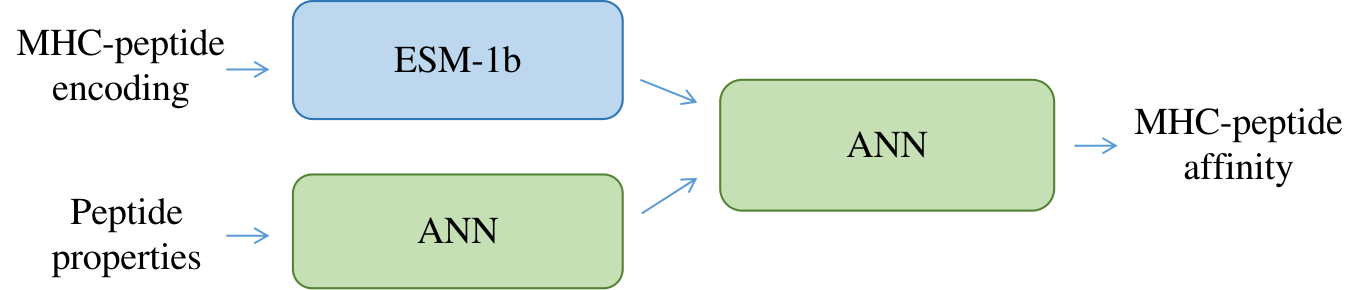
\includegraphics[width=0.9\textwidth]{../img/neoantigen/proposal}	
		\caption{Proceso general utilizado para la detección de neo antígenos a partir de secuencias de DNA. Fuente: \cite{gopanenko2020main}.}
		\label{fig:neo_det_seq}
	\end{figure}
\end{frame}
%-------------------------------------------------------
%-------------------------------------------------------

%-------------------------------------------------------
%-------------------------------------------------------
\begin{frame}{Propuesta}{BERTMHC}	
	\begin{figure}
		\centering
		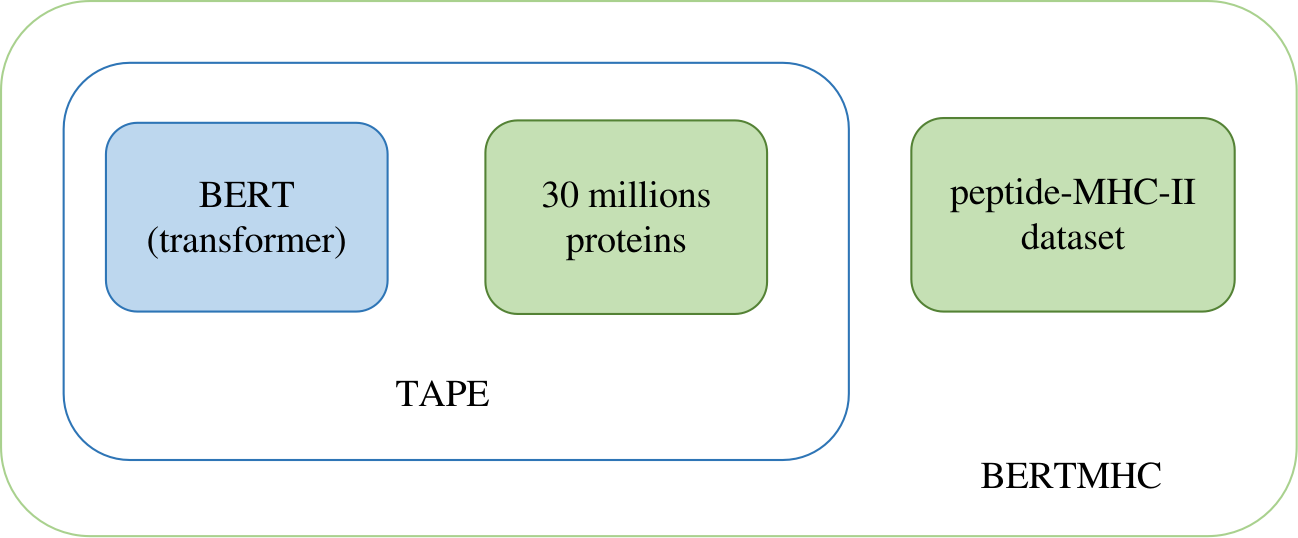
\includegraphics[width=0.9\textwidth]{../img/neoantigen/bertmhc}	
		\caption{BERTMHC.}
	\end{figure}
\end{frame}
%-------------------------------------------------------
%-------------------------------------------------------

%-------------------------------------------------------
%-------------------------------------------------------
\begin{frame}{Propuesta}{APPM}	
	\begin{figure}
		\centering
		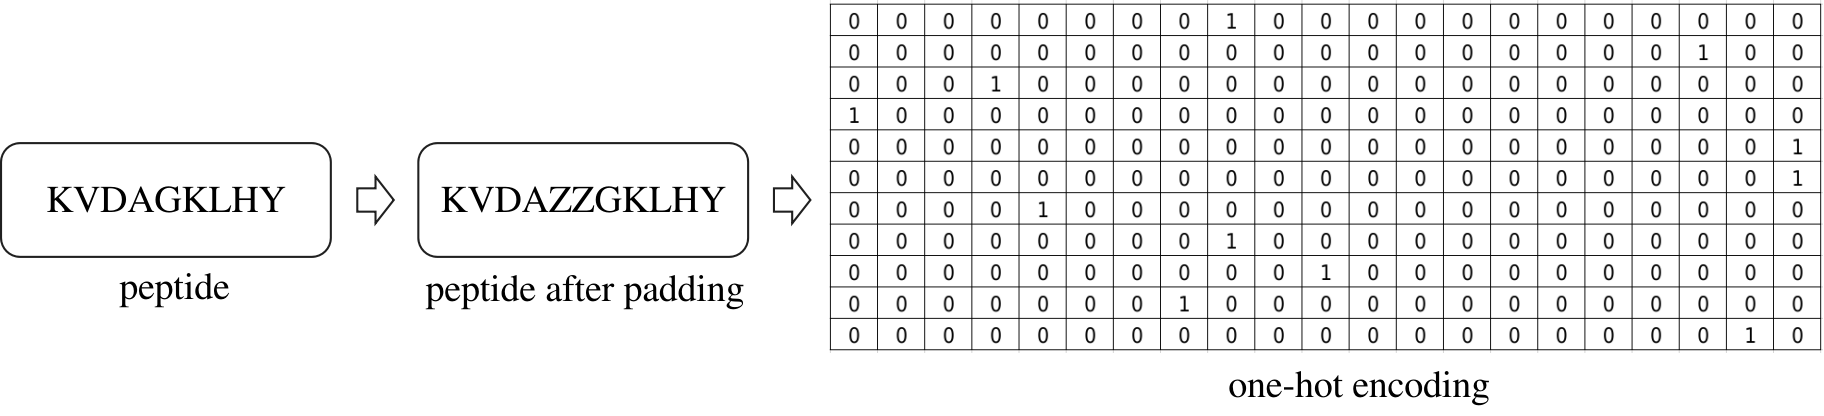
\includegraphics[width=\textwidth]{../img/neoantigen/descriptor}	
		\caption{Proceso para obtener una matriz (imagen) a partir de un péptido (APPM).}
		\label{fig:descriptor}
	\end{figure}
\end{frame}
%-------------------------------------------------------
%-------------------------------------------------------

%%%%%%%%%%%%%%%%%%%%%%%%%%%%%%%%%%%%%%%%%%%%%%%%%%%%%%%%%%%%%%%%%%%%%%%%%%%%%%%%%%%%%%%%%%%%%%%%%%%%%%%%%%%%%%%%
%%%%%%%%%%%%%%%%%%%%%%%%%%%%%%%%%%%%%%%%%%%%%%%%%%%%%%%%%%%%%%%%%%%%%%%%%%%%%%%%%%%%%%
\section{Resultados}
%%%%%%%%%%%%%%%%%%%%%%%%%%%%%%%%%%%%%%%%%%%%%%%%%%%%%%%%%%%%%%%%%%%%%%%%%%%%%%%%%%%%%%%%%%%%%%%%%%%%%%%%%%%%%%%%
%%%%%%%%%%%%%%%%%%%%%%%%%%%%%%%%%%%%%%%%%%%%%%%%%%%%%%%%%%%%%%%%%%%%%%%%%%%%%%%%%%%%%%

%-------------------------------------------------------
%-------------------------------------------------------
\begin{frame}{MHC alleles utilizados}{}
	\begin{table}[h]
		\centering
		\caption{Cantidad de muestras por tipo de \textit{allele}.}
		\label{tab:db}
		\setlength{\tabcolsep}{0.8em} % for the horizontal padding
		{\renewcommand{\arraystretch}{1.3}% for the vertical padding
			\begin{tabular}{ccccc}
				\hline
				\textit{\textbf{Alleles}} & \textbf{Label = 1} & \textbf{Label = 0} & \textbf{Train}  & \textbf{Test}  \\ \hline
				A*01:01                   & 3398               & 48700              & 45498  & 6600  \\ 
				A*02:01                   & 6779               & 165342             & 160921 & 11200 \\ 
				A*02:03                   & 1780               & 116299             & 107879 & 10200 \\ 
				A*31:01                   & 1879               & 45918              & 41597  & 6200  \\ 
				B*44:02                   & 1525               & 44760              & 40085  & 6200  \\ 
				B*44:03                   & 1487               & 39482              & 34769  & 6200  \\ 
				MHC-II alleles            & 1917               & 496                & 1533  & 384  \\ 
			\end{tabular}
		}
	\end{table}
\end{frame}
%-------------------------------------------------------
%-------------------------------------------------------

%-------------------------------------------------------
%-------------------------------------------------------
\begin{frame}{Resultados}{}
\begin{table}[]
	\centering
	\caption{Resultados obtenidos en cada base de datos. }
	\label{tab:results}
	\setlength{\tabcolsep}{0.8em} % for the horizontal padding
	{\renewcommand{\arraystretch}{1.3}% for the vertical padding
		\begin{tabular}{lllll}
			\hline
			\textit{\textbf{Allele}} & \textit{\textbf{Accuracy}} & \textit{\textbf{F1 score}} & \textit{\textbf{Precision}} & \textit{\textbf{Recall}} \\
			\hline
			A*01:01                  & 0.978                      & 0.917                      & 0.982                       & 0.887                    \\
			A*0201                   & 0.962                      & 0.956                      & 0.965                       & 0.948                    \\
			A*02:03                  & 0.992                      & 0.979                      & 0.994                       & 0.969                    \\
			A*31:01                  & 0.980                      & 0.968                      & 0.989                       & 0.951                    \\
			B*44:02                  & 0.991                      & 0.981                      & 0.968                       & 0.997                    \\
			B*44:03                  & 0.992                      & 0.987                      & 0.995                       & 0.980                   
		\end{tabular}
	}
\end{table}
\end{frame}
%-------------------------------------------------------
%-------------------------------------------------------

%-------------------------------------------------------
%-------------------------------------------------------
\begin{frame}{Resultados}{}
	\begin{figure}[H]
		\centering
		\subfigure[A*01:01]{\label{fig:a}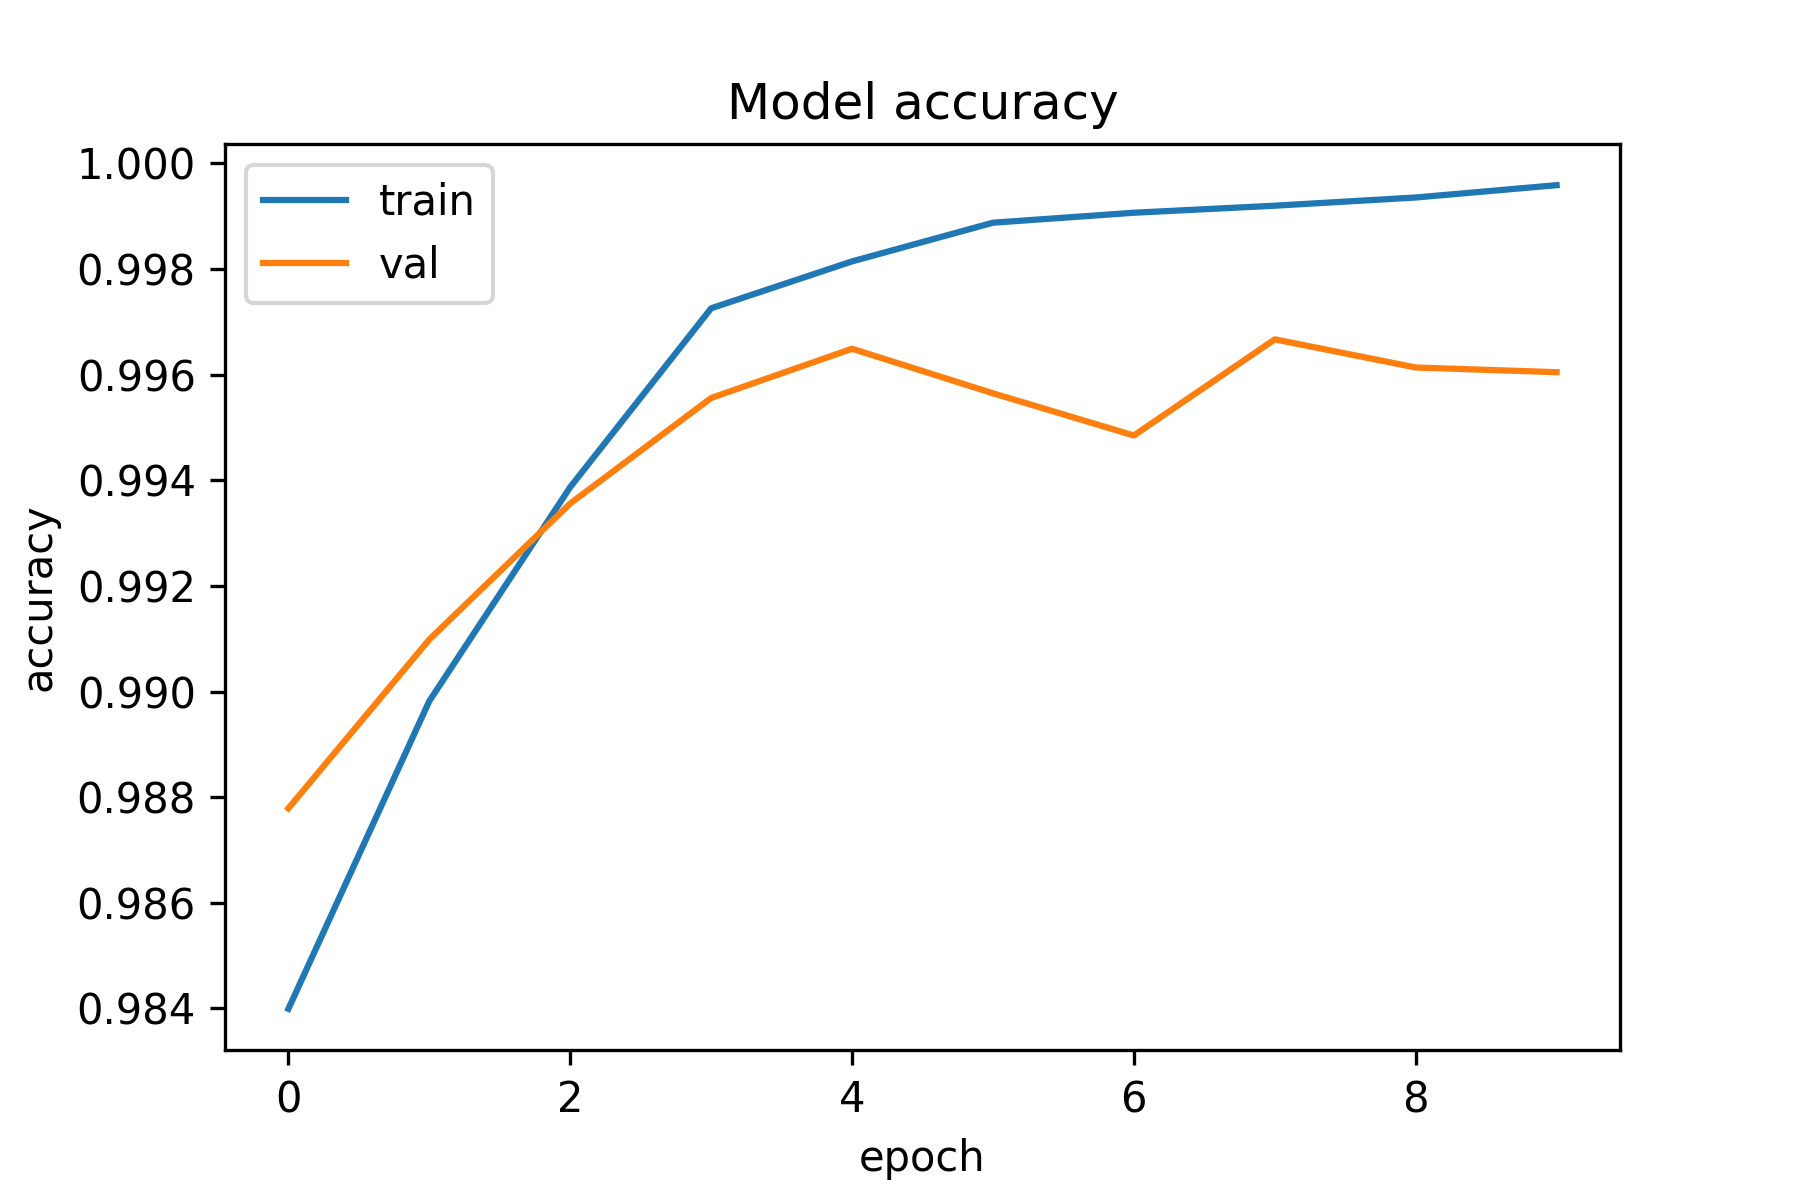
\includegraphics[width=0.35\textwidth]{../img/neoantigen/acc_A0203}}
		\subfigure[A*02:01]{\label{fig:b}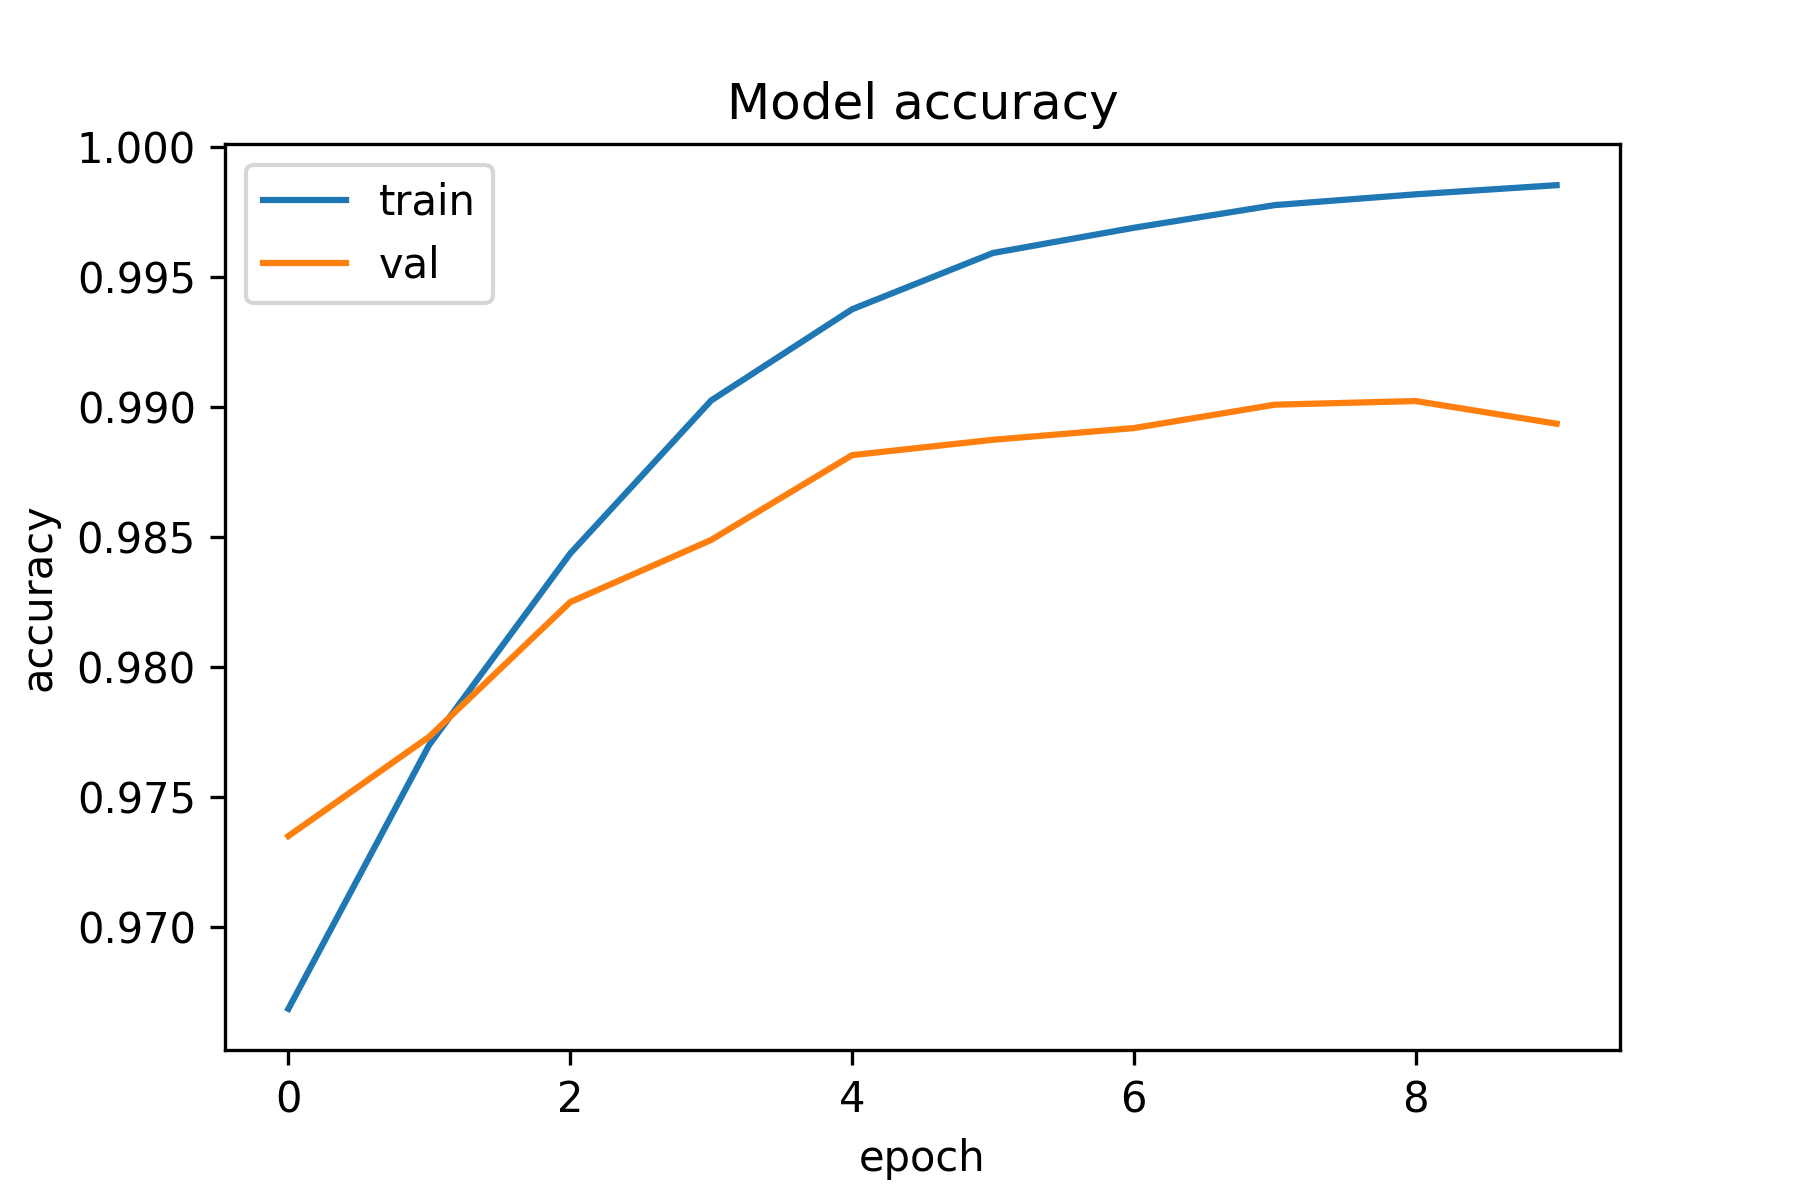
\includegraphics[width=0.35\textwidth]{../img/neoantigen/acc_A0201}}
		\subfigure[A*02:03]{\label{fig:a}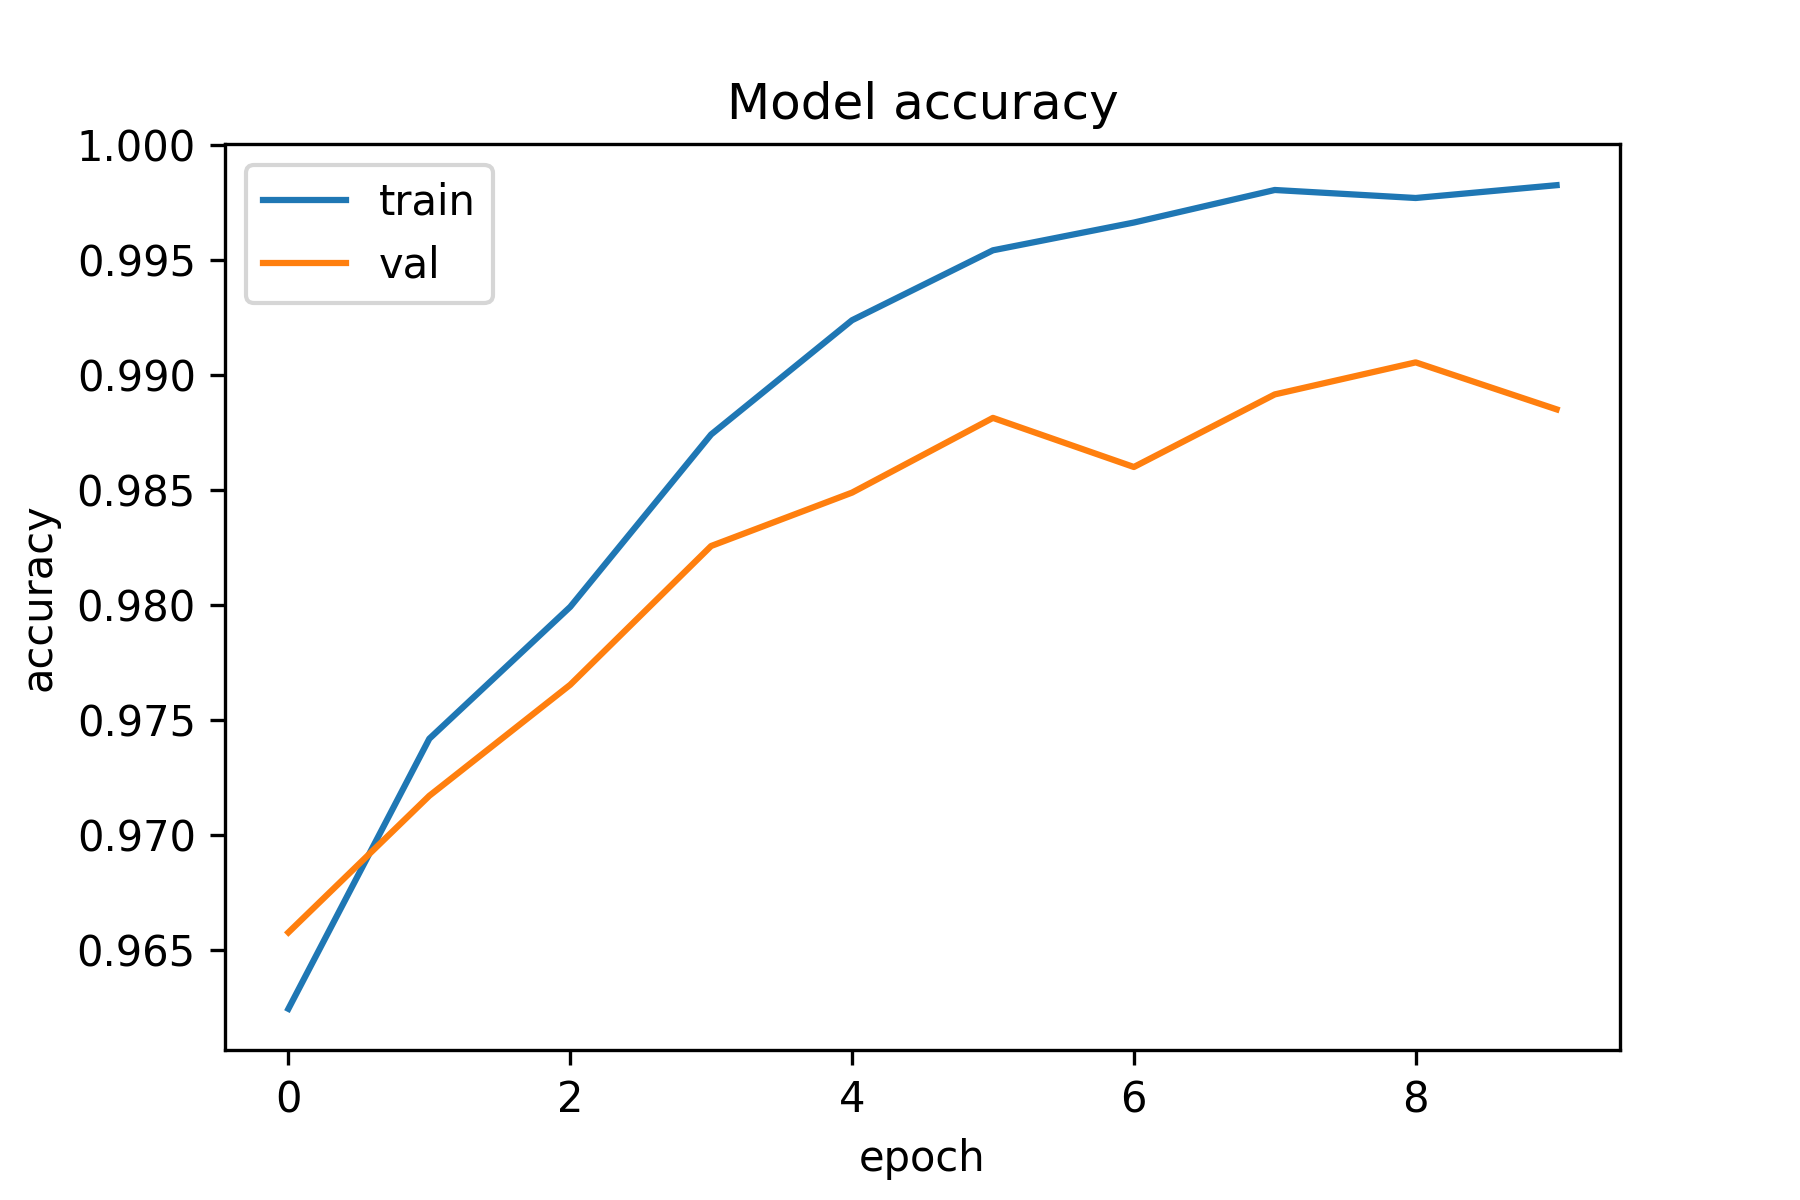
\includegraphics[width=0.35\textwidth]{../img/neoantigen/acc_A0101}}
		\subfigure[A*31:01]{\label{fig:b}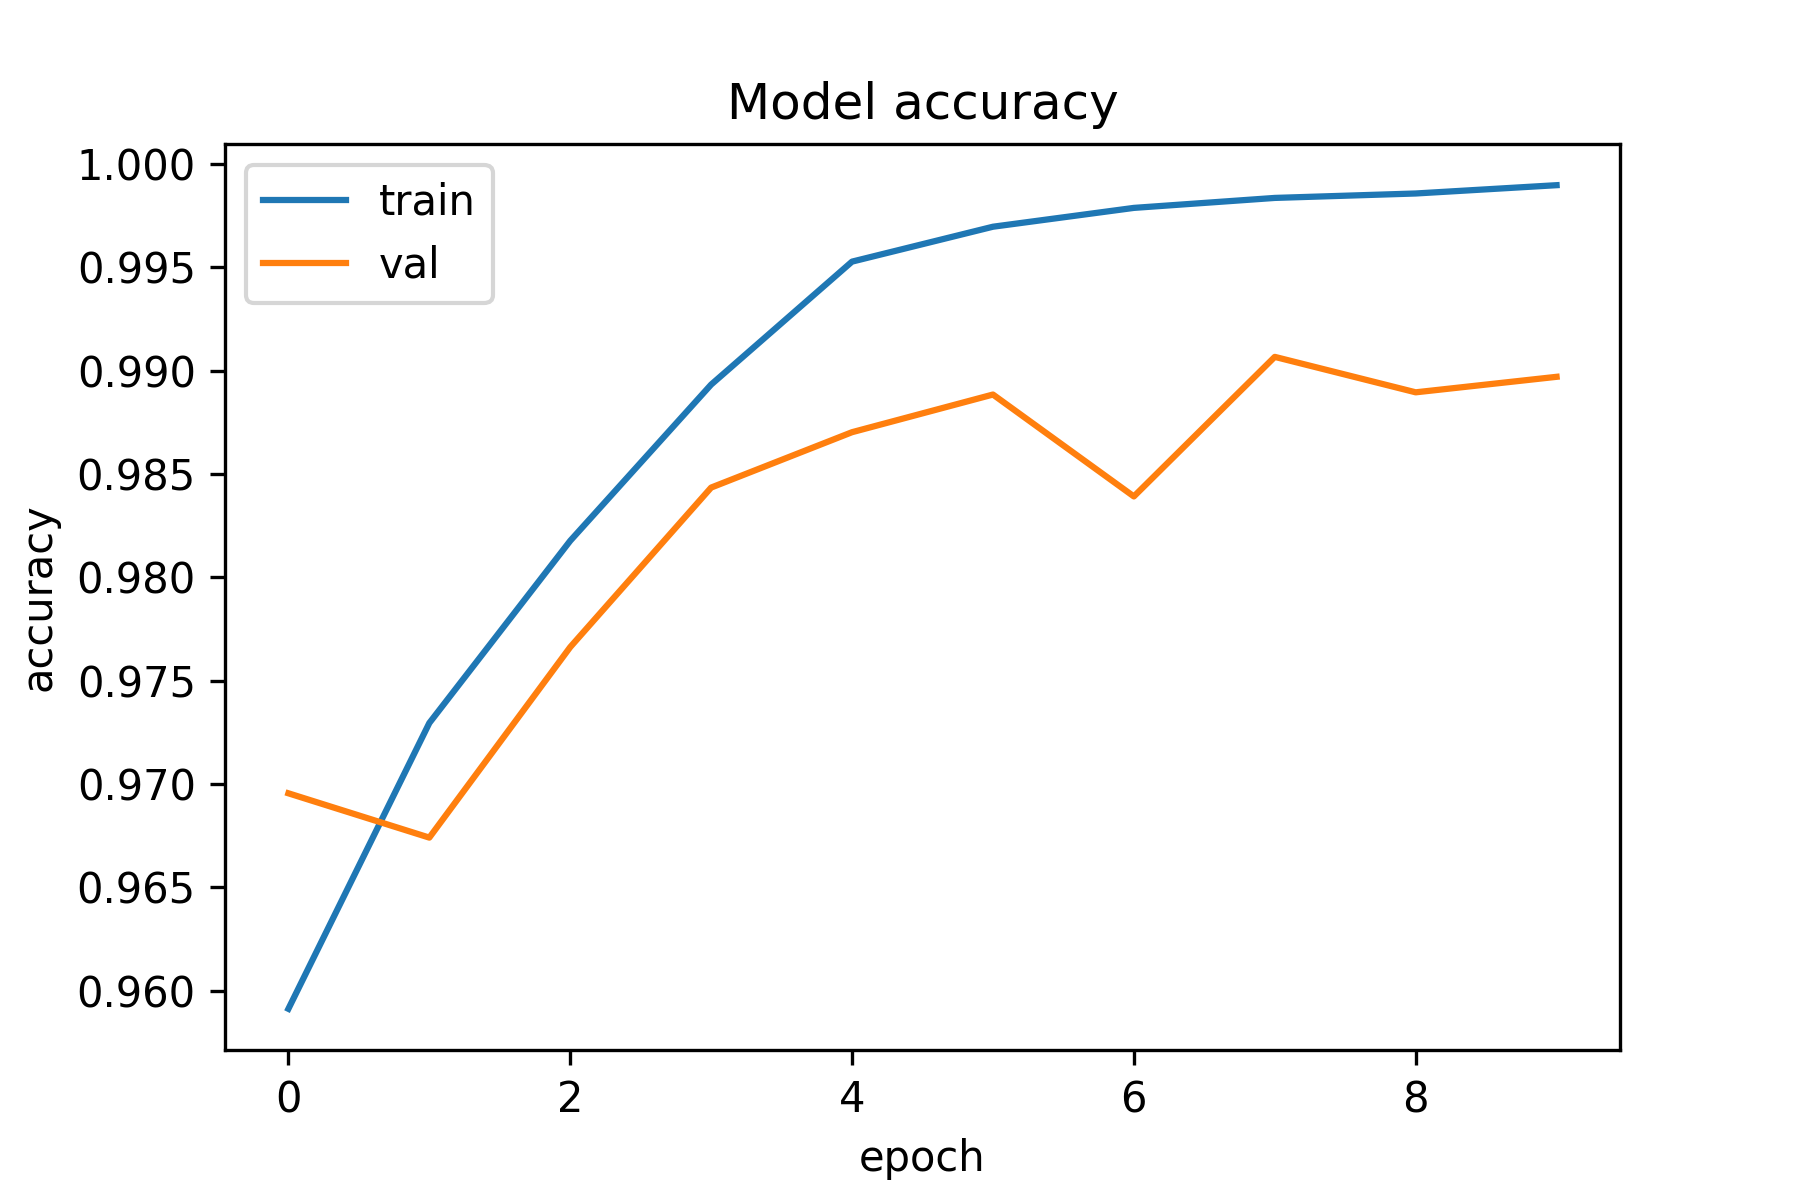
\includegraphics[width=0.35\textwidth]{../img/neoantigen/acc_A3101}}
		%\subfigure[B*44:02]{\label{fig:a}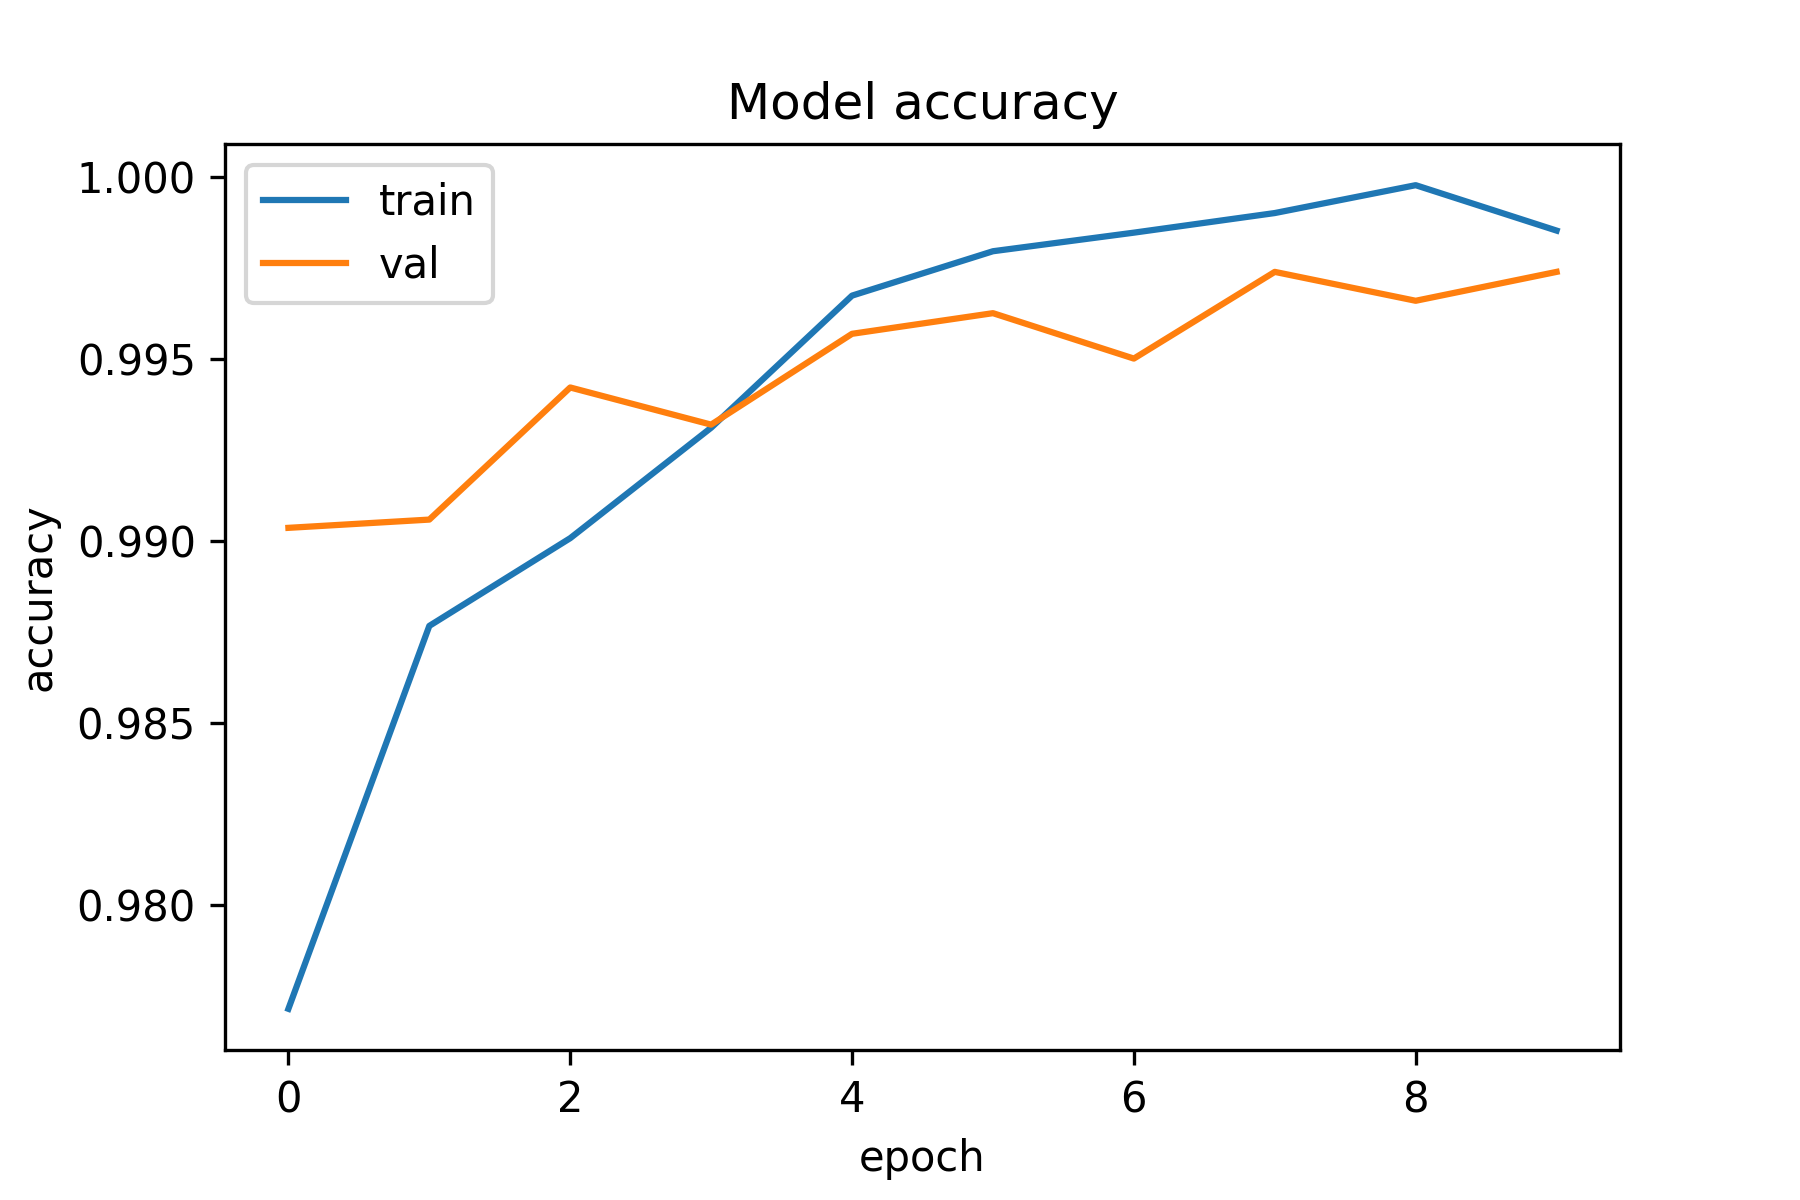
\includegraphics[width=0.4\textwidth]{img/neoantigen/acc_B4402}}
		%\subfigure[B*44:03]{\label{fig:b}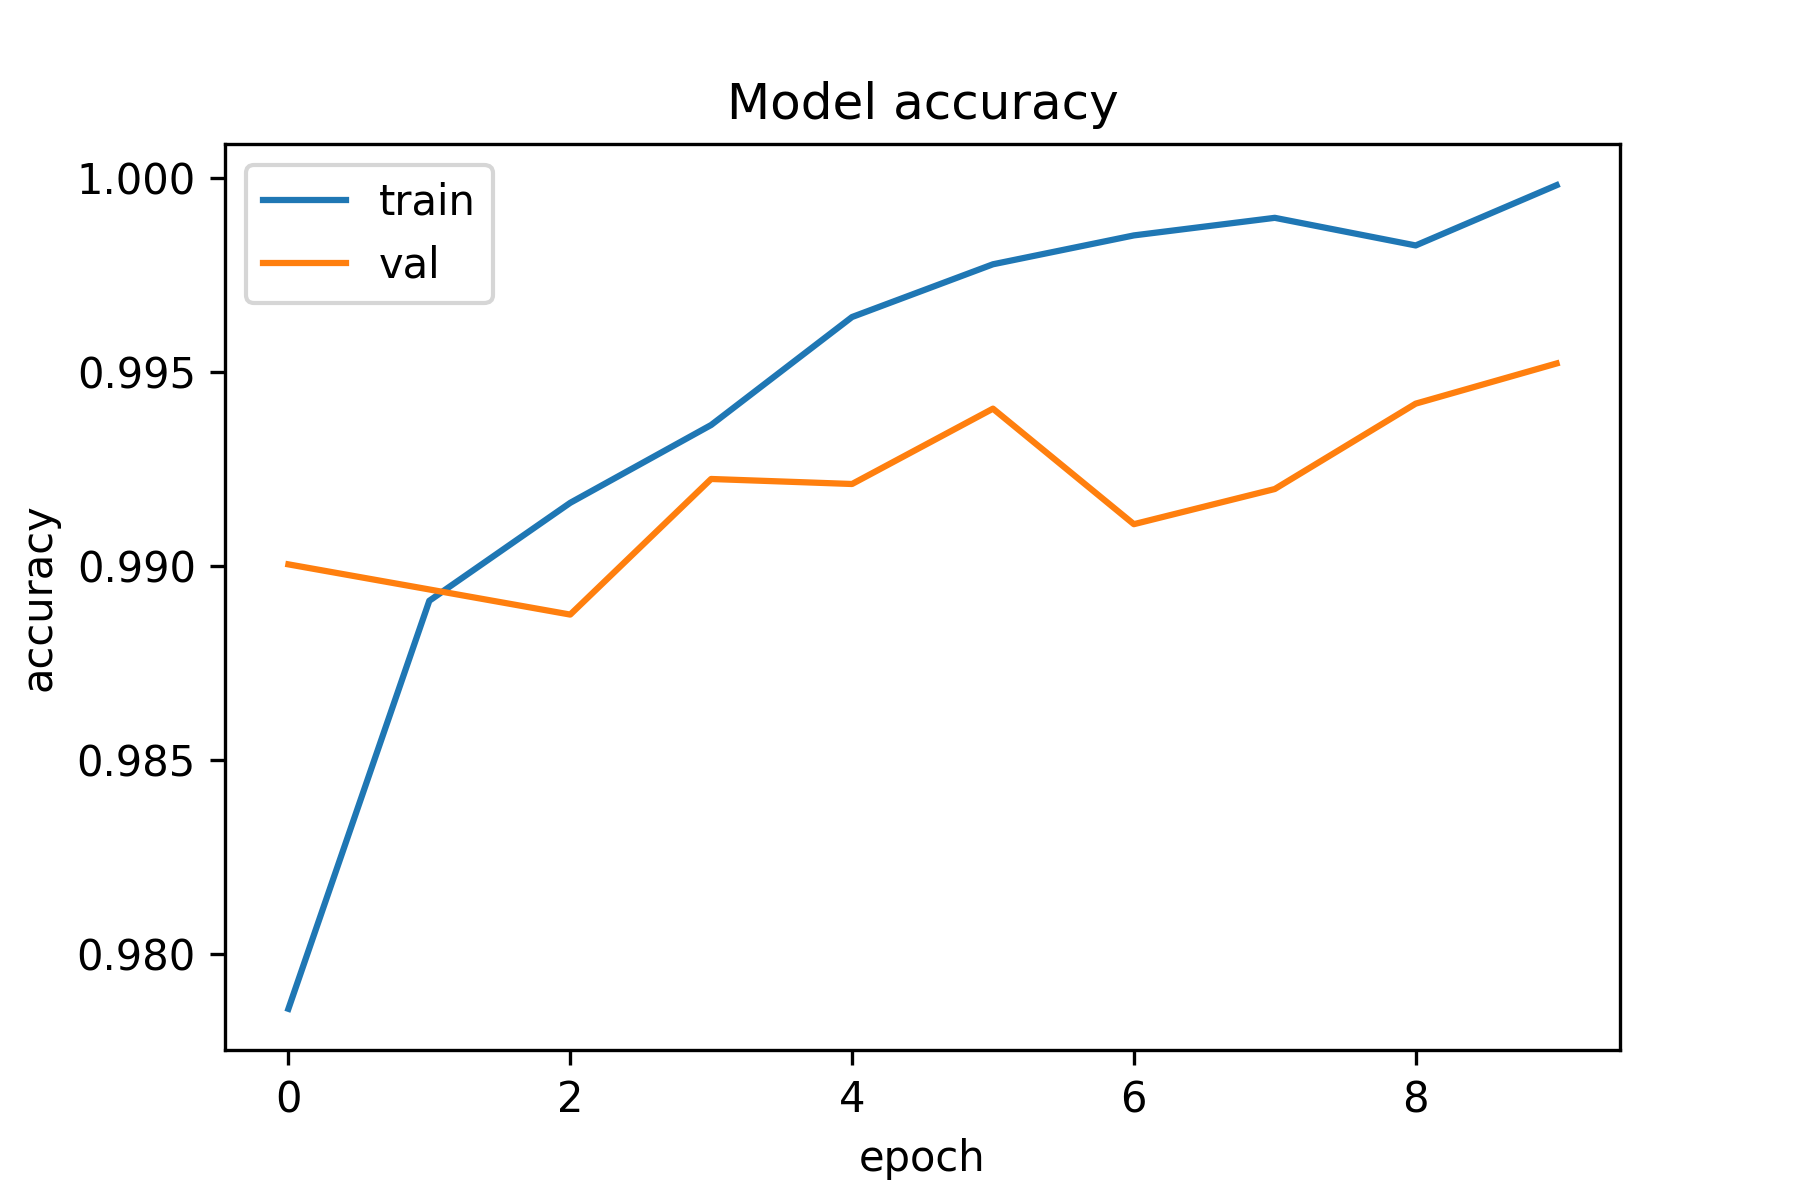
\includegraphics[width=0.4\textwidth]{img/neoantigen/acc_B4403}}		
		
		\caption{\textit{Accuracy} durante cada \textit{epoch}, para cada base de datos. Las bases de datos representan las células HLA A*01:01, A*02:01, A*02:03, A*31:01.}
		\label{fig:result}
	\end{figure}
\end{frame}
%-------------------------------------------------------
%-------------------------------------------------------




%%%%%%%%%%%%%%%%%%%%%%%%%%%%%%%%%%%%%%%%%%%%%%%%%%%%%%%%%%%%%%%%%%%%%%%%%%%%%%%%%%%%%%%%%%%%%%%%%%%%%%%%%%%%%%%%
%%%%%%%%%%%%%%%%%%%%%%%%%%%%%%%%%%%%%%%%%%%%%%%%%%%%%%%%%%%%%%%%%%%%%%%%%%%%%%%%%%%%%%
\section{Conclusiones y Trabajos futuros}
%%%%%%%%%%%%%%%%%%%%%%%%%%%%%%%%%%%%%%%%%%%%%%%%%%%%%%%%%%%%%%%%%%%%%%%%%%%%%%%%%%%%%%%%%%%%%%%%%%%%%%%%%%%%%%%%
%%%%%%%%%%%%%%%%%%%%%%%%%%%%%%%%%%%%%%%%%%%%%%%%%%%%%%%%%%%%%%%%%%%%%%%%%%%%%%%%%%%%%%


%-------------------------------------------------------
%-------------------------------------------------------
\begin{frame}{Conclusiones}{}
	
	\begin{block}{}
		Se ha desarrollado una RSL, sobre los métodos de detección de neoantígenos utilizando \textit{deep learning}. Esto ha logrado identificar las tendencias, retos y problemas del tema de interes.
	\end{block}

	\begin{block}{}
		Se ha realizado experimentos preliminares, sobre el uso de CNNs para el problema de peptide-MHC presentation. Se ha utilizado muestras de MS con un enfoque \textit{single allele} (se entrena varios modelos para cada tipo de MHC). 
	\end{block}

\end{frame}
%-------------------------------------------------------
%-------------------------------------------------------


%-------------------------------------------------------
%-------------------------------------------------------
\begin{frame}{Trabajos futuros}{}
	\begin{block}{}
		Recientemente un trabajo \cite{hashemi2022improved} tambien propone el uso de \textit{transfer learning} pero de un modelo pre-entrenado con 250 millones de proteínas. Entonces, se plantea utilizar la misma red, aumentar la cantidad de muestras y evaluar los resultados.
	\end{block}
	
	\begin{block}{}
		Actualmente se cuenta con una base de datos de proteínas MHC \cite{e2019phla3d}, entonces utilizando AlphaFold de Google, se plantea predecir la estructura de varios péptidos y analizar el enlace péptido-MHC desde un punto de vista de la computación gráfica.	
	\end{block}
	
	
\end{frame}
%-------------------------------------------------------
%-------------------------------------------------------

%-------------------------------------------------------
%-------------------------------------------------------
\begin{frame}[allowframebreaks]
	\frametitle{References}
	%\bibliographystyle{amsalpha}
	\bibliographystyle{IEEEtran}
	\bibliography{../bibliography_thesis.bib}
\end{frame}
%-------------------------------------------------------
%-------------------------------------------------------

%-------------------------------------------------------
%-------------------------------------------------------
\if\mycmd1 % MY THEME
\1{
	{\1
		\begin{frame}[plain,noframenumbering]
			%\finalpage{Thank you}
			\begin{figure}[]
				\centering
				
\includegraphics[width=\textwidth,height=0.7\textheight,keepaspectratio]{img/question.png}
				%\label{img:mot2}
				%\caption{Image example in 2 gray levels.}
			\end{figure}
	\end{frame}}
	\else % CS THEME
	\begin{frame}{Questions?}
		\begin{figure}[]
			\centering
			
\includegraphics[width=\textwidth,height=0.7\textheight,keepaspectratio]{img/question.png}
			%\label{img:mot2}
			%\caption{Image example in 2 gray levels.}
		\end{figure}
		
	\end{frame}
	\fi
	%-------------------------------------------------------
	%-------------------------------------------------------
	

\end{document}